\documentclass[conference, onecolumn]{IEEEtran}
\IEEEoverridecommandlockouts
% The preceding line is only needed to identify funding in the first footnote. If that is unneeded, please comment it out.
\usepackage[a4paper, top=3cm, bottom=3cm, left=2.5cm, right=2.5cm]{geometry}
\usepackage{graphicx}
\usepackage{amsmath}
\usepackage{booktabs}
\usepackage{parskip}
\setlength{\parindent}{0pt}
\usepackage[T1]{fontenc}
\usepackage{lmodern}
\usepackage{hyperref}
\usepackage{multirow}
\usepackage{amssymb}
\usepackage{listings}
\usepackage{float}
\usepackage{subcaption}
\hypersetup{colorlinks=true, linkcolor=black, urlcolor=blue, citecolor=black}
 

\usepackage{tabularx} % For auto-adjusting column widths

\def\BibTeX{{\rm B\kern-.05em{\sc i\kern-.025em b}\kern-.08em
    T\kern-.1667em\lower.7ex\hbox{E}\kern-.125emX}}
\begin{document}
\pagestyle{plain}       % Enables page numbers globally
\thispagestyle{empty}   % Suppresses the page number on this first page




%\begin{titlepage}
\begin{center}
\vspace{4cm}
%\textsc{ Danmarks Tekniske Universitet}\\[1.5cm]

\includegraphics[width=0.4\textwidth]{dtu.png}~\\[1cm]
\vspace{2cm}

\vspace{2cm}

% Title
\hrule
\vspace{.5cm}
{ \huge \bfseries 02443 Stochastic Simulation, Summer 2026\\
Exercises - Group 67} % title of the report
\vspace{.5cm}

\hrule
\vspace{1.5cm}

\textsc{\textbf{Authors}}\\
\vspace{.2cm}
\centering

% add your name here
Linus Juni\\
StudentID: s676767\\

\vspace{2mm}
Theodor Dornonville de la Cour\\
StudentID: s225093\\

\vspace{2mm}
Mathilde Brinch Sørensen\\
StudentID: s254124\\

\vspace{2mm}
Mathias Markvardsen\\
StudentID: s225182


\vspace{3cm}

\centering \today % Todays date
\end{center}
\section*{GenAI Declaration}
We have used artificial intelligence tools from OpenAI, Anthropic, and Google for coding and to assist with writing. In accordance with DTU’s guidelines for documenting the use of Generative AI, we acknowledge this usage.

\newpage
\newpage
\section*{Day 1 exercises}

In this exercise we implement a pseudorandom number generator
from scratch and assess its statistical quality. We use a
\textbf{Linear Congruential Generator (LCG)}, defined by the recurrence
\begin{equation}
    x_i = (a \cdot x_{i-1} + c) \bmod M, \qquad U_i = \frac{x_i}{M},
    \label{eq:lcg}
\end{equation}
where $a$ is the multiplier, $c$ is the increment, $M$ is the modulus, and
$x_0$ is the seed. The values $U_i \in [0, 1)$ serve as approximations to
independent uniform random variables, and their quality depends entirely on
the choice of parameters. We evaluate quality using four tests at the 5\%
significance level with $n = 10{,}000$ samples, summarised in
Table~\ref{tab:critical}.

\begin{table}[h]
    \centering
    \caption{Critical values for the four statistical tests at the 5\% level.}
    \label{tab:critical}
    \renewcommand{\arraystretch}{1.1}
    \begin{tabular}{ll}
        \toprule
        Test & Reject $H_0$ if \\
        \midrule
        Chi-square ($k = 10$ bins) & $T > 16.9$ \\
        Kolmogorov--Smirnov        & $D > 0.0136$ \\
        Runs                       & $|Z| > 1.96$ \\
        Pearson serial corr.\      & $|r_h| > 1.96/\sqrt{n} \approx 0.020$ \\
        $c_h$ test (lecture)       & $|Z_h| > 1.96$,\quad $Z_h = (c_h - \tfrac{1}{4})\big/\sqrt{7/(144n)}$ \\
        \bottomrule
    \end{tabular}
\end{table}

% ================================================================
\section*{Part 1a -- Generating Numbers and Histogram}
% ================================================================

We generate $n = 10{,}000$ values from the LCG in Equation~\eqref{eq:lcg}
using the parameters $a = 1{,}664{,}525$, $c = 1{,}013{,}904{,}223$, and
$M = 2^{32}$ -- a quick Google search reveals these come from
\textit{Numerical Recipes in C} (Press et al., 1992) -- displayed in a histogram with $k = 10$ equal-width bins over
$[0, 1)$. Under uniformity, each bin should contain approximately
$n/k = 1{,}000$ values. As seen in Figure~\ref{fig:histograms} (left), the
histogram is visually flat, providing an initial indication that the
generator produces uniform output.

% ================================================================
\section*{Part 1b -- Statistical Quality Tests}
% ================================================================

We evaluate the good LCG using all tests. The results are summarised in
Table~\ref{tab:good_system} (left), and the lag-1 scatter plot is shown in
Figure~\ref{fig:scatters} (left). The uniformity and runs tests pass
comfortably. For serial correlation we apply two methods: the Pearson
autocorrelation coefficient $r_h$ and the lecture's $c_h$ statistic
($c_h = \frac{1}{n-h}\sum U_i U_{i+h}$, expected $\tfrac{1}{4}$ under
$H_0$). The NR LCG passes the Pearson test at all lags, but the $c_h$ test
rejects at lags 1 and 5, indicating subtle product-moment structure that
centred correlation misses. The scatter plot is visually structureless,
confirming the effect is small in magnitude.

% ================================================================
\section*{Part 1c -- Bad vs.\ Good Parameters}
% ================================================================

To illustrate how critically output quality depends on parameter choice, we
compare two configurations:
\begin{itemize}
    \item \textbf{Bad LCG:} $a = 5$, $c = 1$, $M = 16$ -- a period of only
          16, causing the sequence to cycle in a fixed, predictable order.
    \item \textbf{Good LCG (final choice):} $a = 1{,}664{,}525$,
          $c = 1{,}013{,}904{,}223$, $M = 2^{32}$ -- satisfies the
          Hull--Dobell conditions, guaranteeing a full period of $M$.
\end{itemize}

As shown in Figures~\ref{fig:histograms} and~\ref{fig:scatters} (right
panels), the bad LCG produces a heavily non-uniform histogram and a starkly
structured scatter plot, both direct consequences of the period of 16.
Table~\ref{tab:comparison} confirms this quantitatively: the chi-square
statistic is roughly 100 times the critical value, the runs $Z$-score of 75
is essentially impossible under true randomness, and the lag-1 correlation
of 0.647 confirms that each value strongly predicts the next. The good LCG
passes all tests and is adopted as our final choice.

\begin{figure}[h]
    \centering
    
\includegraphics[width=0.49\textwidth]{plots/day1/good_lcg_histogram.png}
    \hfill
    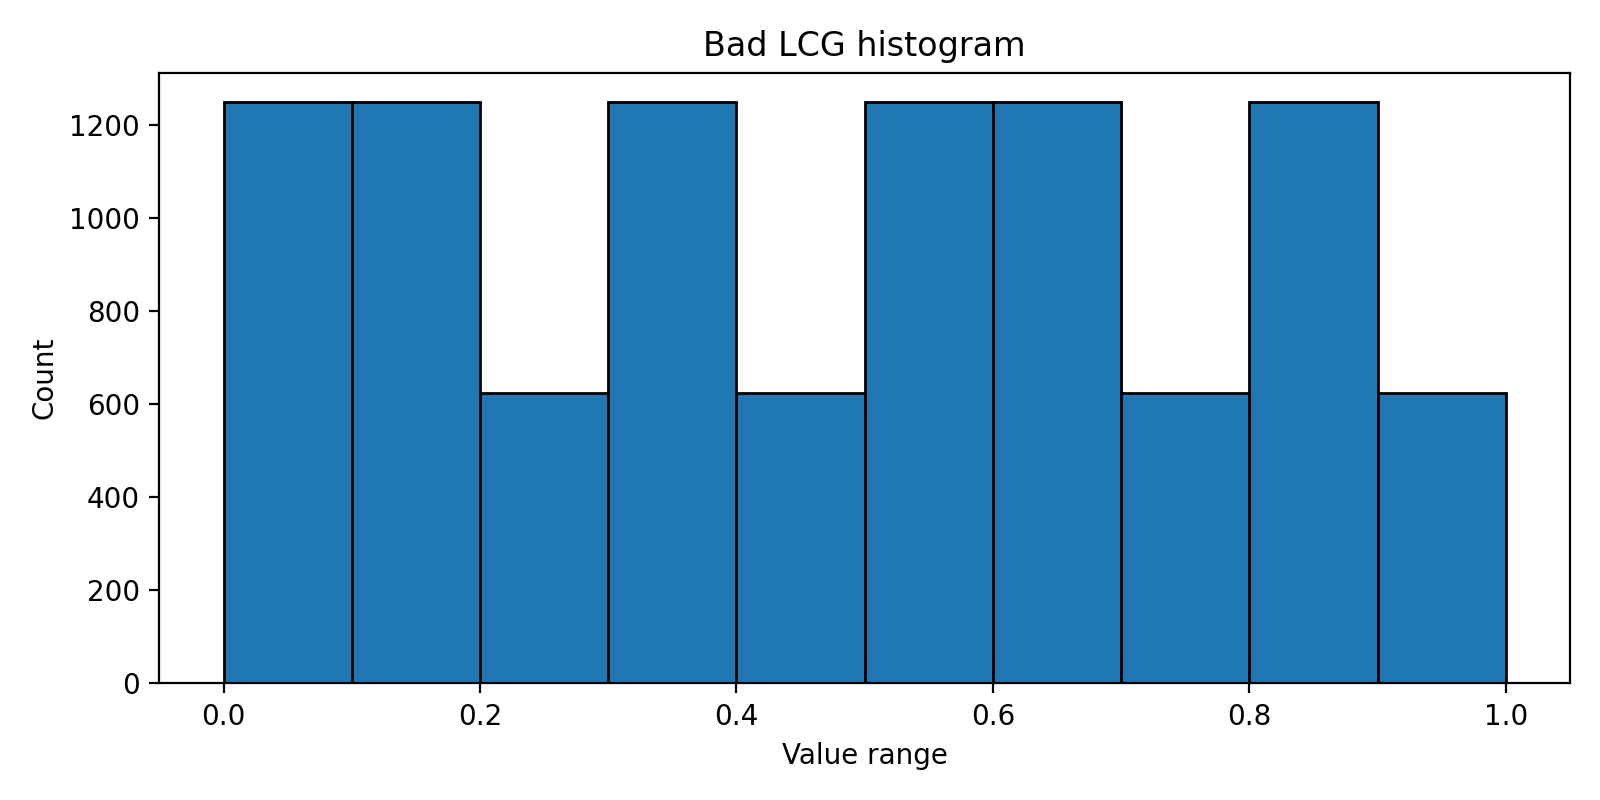
\includegraphics[width=0.49\textwidth]{plots/day1/bad_lcg_histogram.png}
    \caption{Histograms with 10 bins, $n = 10{,}000$.
             \textit{Left:} Good LCG -- counts flat around the expected
             1{,}000 per bin.
             \textit{Right:} Bad LCG -- values concentrate in only 16
             discrete levels ($T = 937.50 \gg 16.9$).}
    \label{fig:histograms}
\end{figure}

\begin{figure}[h]
    \centering
    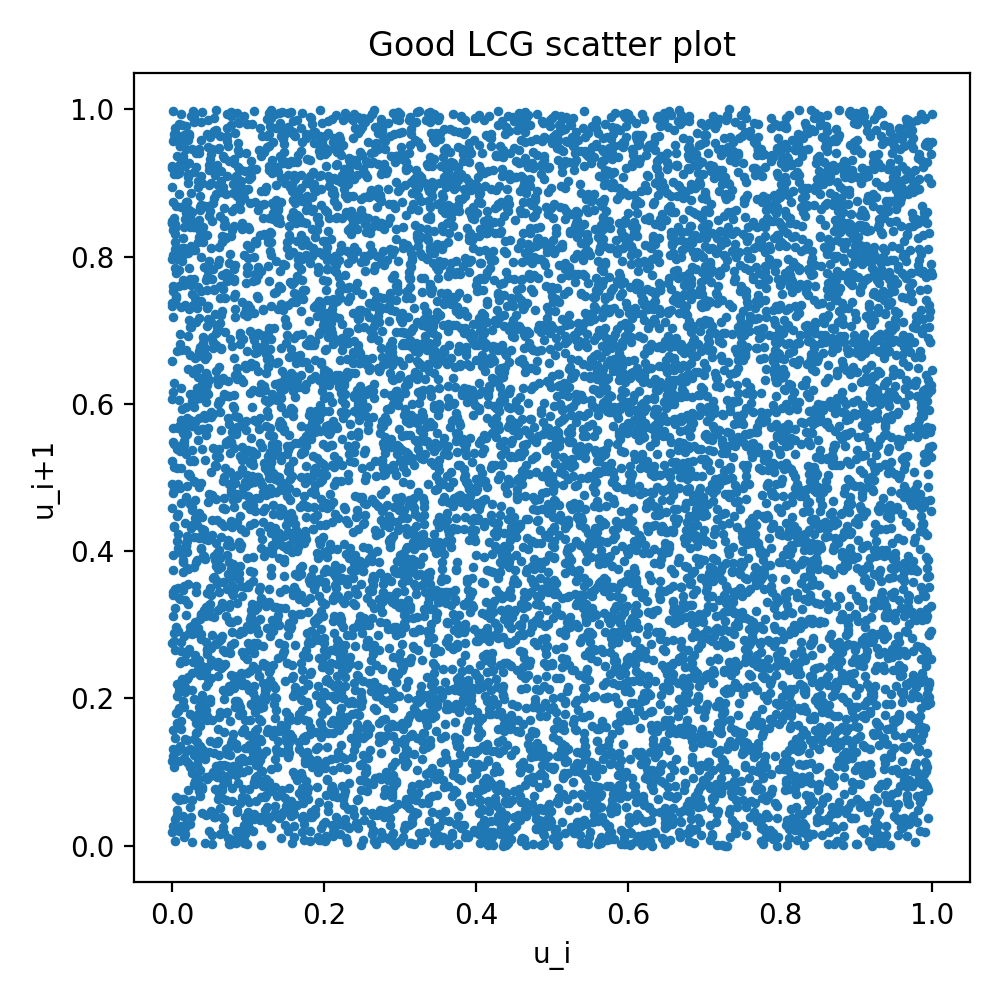
\includegraphics[width=0.49\textwidth]{plots/day1/good_lcg_scatter.png}
    \hfill
    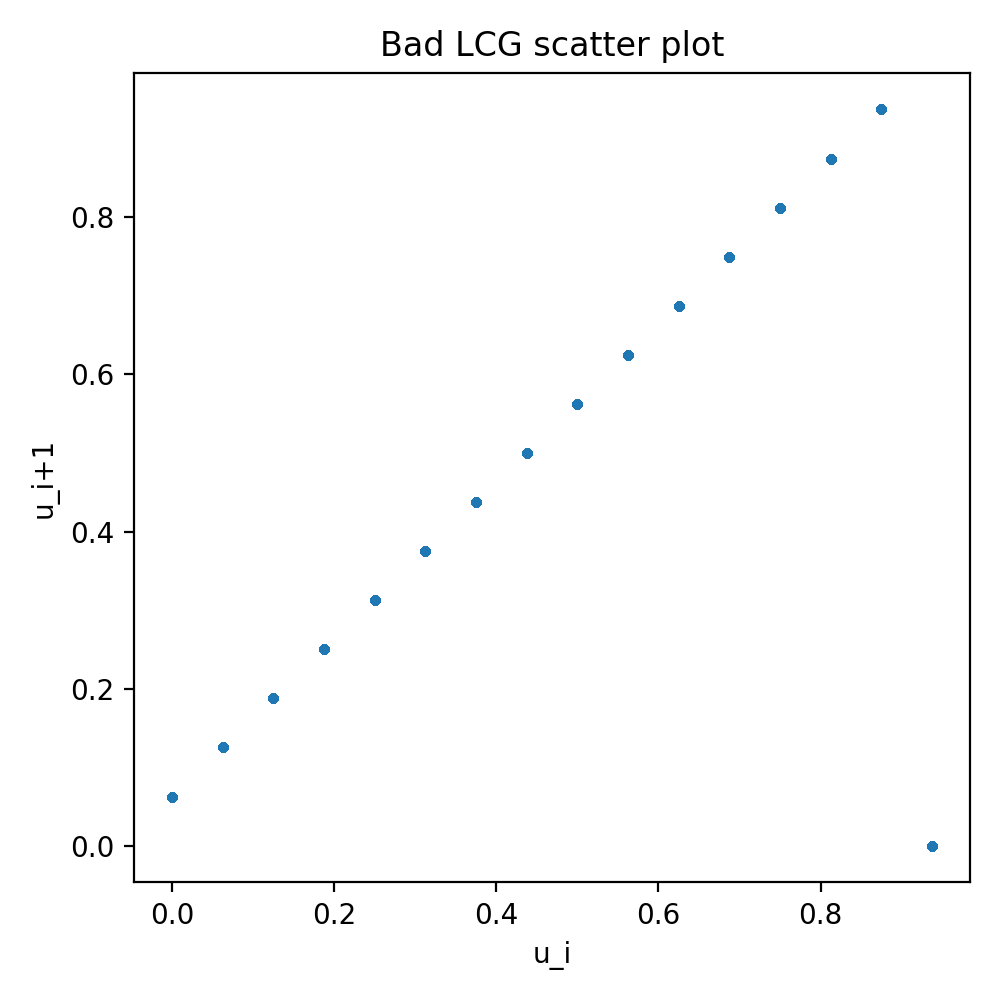
\includegraphics[width=0.49\textwidth]{plots/day1/bad_lcg_scatter.png}
    \caption{Lag-1 scatter plots ($U_i$ vs.\ $U_{i+1}$), $n = 10{,}000$.
             \textit{Left:} Good LCG -- structureless cloud, consistent with
             independence.
             \textit{Right:} Bad LCG -- regular grid structure reflecting the
             deterministic 16-value cycle (lag-1 corr.\ $= 0.647$).}
    \label{fig:scatters}
\end{figure}

\begin{table}[h]
    \centering
    \caption{Statistical test results for the bad vs.\ good LCG
             ($n = 10{,}000$; critical values at the 5\% level in brackets).}
    \label{tab:comparison}
    \renewcommand{\arraystretch}{1.1}
    \begin{tabular}{lrcrc}
        \toprule
        Test & Bad LCG & & Good LCG & \\
        \midrule
        Chi-square {[}$< 16.9${]}  & $937.50$ & $\times$ & $9.65$   & \checkmark \\
        KS {[}$< 0.0136${]}        & $0.0625$ & $\times$ & $0.0093$ & \checkmark \\
        Runs $|Z|$ {[}$< 1.96${]}  & $75.02$  & $\times$ & $1.22$   & \checkmark \\
        Corr $h = 1$               & $0.647$  & $\times$ & $0.007$  & \checkmark \\
        Corr $h = 2$               & $0.341$  & $\times$ & $-0.003$ & \checkmark \\
        Corr $h = 5$               & $-0.294$ & $\times$ & $-0.009$ & \checkmark \\
        \bottomrule
    \end{tabular}
\end{table}

% ================================================================
\section*{Part 2 -- System Generator}
% ================================================================

We apply the same test suite to Python's built-in \texttt{random} module,
which uses the Mersenne Twister with period $2^{19937} - 1$. The results for
a single seed are shown alongside the good LCG in Table~\ref{tab:good_system},
and the corresponding histogram and scatter plot in
Figure~\ref{fig:sys_hist_scatter}. The Mersenne Twister passes all tests,
including both the Pearson and $c_h$ serial correlation tests, whereas the
NR LCG fails the $c_h$ test at lags 1 and 5. The $c_h$ statistic is more
sensitive here because it tests the raw product moment $E[U_i U_{i+h}]$
rather than the centred covariance, and thereby detects slight systematic
shifts in the joint distribution that Pearson correlation misses.

\begin{figure}[h]
    \centering
    
\includegraphics[width=0.49\textwidth]{plots/day1/system_histogram.png}
    \hfill
    
\includegraphics[width=0.49\textwidth]{plots/day1/system_scatter.png}
    \caption{Mersenne Twister system generator, $n = 10{,}000$.
             \textit{Left:} Histogram with 10 bins; visually flat, consistent
             with uniformity.
             \textit{Right:} Lag-1 scatter plot; no visible structure,
             consistent with independence.}
    \label{fig:sys_hist_scatter}
\end{figure}

\begin{table}[h]
    \centering
    \caption{Test results for the good LCG and Mersenne Twister
             ($n = 10{,}000$, seed $= 67$; critical values at the 5\% level
             in brackets).}
    \label{tab:good_system}
    \renewcommand{\arraystretch}{1.1}
    \begin{tabular}{lrcrc}
        \toprule
        Test & Good LCG & & Mersenne Twister & \\
        \midrule
        Chi-square {[}$< 16.9${]}           & $12.61$ & \checkmark & $7.76$   & \checkmark \\
        KS {[}$< 0.0136${]}                 & $0.0120$ & \checkmark & $0.0084$ & \checkmark \\
        Runs $|Z|$ {[}$< 1.96${]}           & $1.00$  & \checkmark & $0.20$   & \checkmark \\
        \midrule
        Pearson $r_1$ {[}$< 0.020${]}       & $-0.018$ & \checkmark & $-0.006$ & \checkmark \\
        Pearson $r_2$                        & $+0.005$ & \checkmark & $+0.012$ & \checkmark \\
        Pearson $r_5$                        & $-0.010$ & \checkmark & $-0.004$ & \checkmark \\
        \midrule
        $c_h$ test $h=1$ {[}$|Z|< 1.96${]} & $-3.19$  & $\times$   & $0.38$   & \checkmark \\
        $c_h$ test $h=2$                    & $-2.34$  & $\times$   & $-0.36$  & \checkmark \\
        $c_h$ test $h=5$                    & $-2.87$  & $\times$   & $-1.09$  & \checkmark \\
        \bottomrule
    \end{tabular}
\end{table}

% ================================================================
\section*{Part 3 -- Sufficiency of a Single Sample}
% ================================================================

Each test statistic is itself a random variable, so a single sample
represents only one realisation. An unlucky seed can cause a good generator
to marginally fail a test, while a lucky seed can make a poor one look
acceptable. To obtain a reliable characterisation, we repeat each test over
100 independent seeds and record the \emph{rejection rate} -- the fraction
of seeds for which $H_0$ is rejected at the 5\% level. For a perfectly
calibrated test applied to a good generator this rate should be close to 5\%.
The results are shown in Table~\ref{tab:multiseed}. The uniformity and runs
tests look reasonable for both generators ($\approx 4$--$6\%$, close to the
expected 5\%). The $c_h$ correlation test is a different story -- it rejects
at $15$--$17\%$ for \emph{both} generators, which seems too high. Interestingly,
this happens for the Mersenne Twister just as much as for the NR LCG, which
suggests the issue is with the test itself rather than either generator. One
possible explanation is that the variance formula $7/(144n)$ is only an
approximation and may underestimate the true variance, causing the test to
reject too often. We are not entirely sure, but the pattern is suspicious
enough that we would not put too much weight on the single-seed $c_h$ failures
seen for the NR LCG earlier. We conclude that a single sample is insufficient
for a reliable assessment.

\begin{table}[h]
    \centering
    \caption{Rejection rates (\%) over 1{,}000 seeds for the good LCG and the
             Mersenne Twister ($n = 10{,}000$ per seed; expected $\approx 5\%$
             for a well-calibrated test).}
    \label{tab:multiseed}
    \renewcommand{\arraystretch}{1.1}
    \begin{tabular}{lrr}
        \toprule
        Test                  & Good LCG & Mersenne Twister \\
        \midrule
        Chi-square            & $6.1\%$  & $4.6\%$ \\
        KS                    & $6.0\%$  & $5.4\%$ \\
        Runs                  & $4.5\%$  & $4.6\%$ \\
        $c_h$ test $h = 1$    & $15.4\%$ & $17.5\%$ \\
        $c_h$ test $h = 2$    & $17.1\%$ & $15.9\%$ \\
        $c_h$ test $h = 5$    & $16.5\%$ & $15.5\%$ \\
        \bottomrule
    \end{tabular}
\end{table}

% ================================================================
\section*{Conclusion}
\addcontentsline{toc}{section}{Conclusion}
% ================================================================

We implemented a Linear Congruential Generator and demonstrated that
parameter choice is critical to its quality. The bad generator with
$a = 5$, $c = 1$, $M = 16$ fails all statistical tests catastrophically
due to its period of only 16. The good generator with
$a = 1{,}664{,}525$, $c = 1{,}013{,}904{,}223$, $M = 2^{32}$ passes the
uniformity, runs, and Pearson autocorrelation tests. The lecture's $c_h$
test rejects it at short lags on the chosen seed, but the multi-seed
analysis shows this is consistent with the test's elevated false positive
rate ($\approx 16\%$) caused by an approximation in the variance formula
-- Python's Mersenne Twister shows the same inflation. The uniformity and
runs tests behave correctly ($\approx 5\%$) for both generators. Finally,
we showed that a single sample is insufficient for reliable assessment, and
that tracking rejection rates across many seeds is the appropriate action.
\newpage
\newpage
\section*{Day 2 exercises}

In these exercises we transform a supply of $U \sim \mathcal{U}(0,1)$
variates from Day 1 into random variables $X$ with a prescribed distribution
function $F$, covering both discrete and continuous cases.
All simulations use $n = 10{,}000$ observations unless stated otherwise.

\section*{Exercise 2 --- Discrete Distributions}

% ================================================================
\section*{Part 1 --- Geometric Distribution}
% ================================================================

The Geometric($p$) distribution models the number of trials needed to get
the first success, where each trial succeeds independently with probability
$p$. The theoretical mean is $1/p$. As an example, if success has a 10\% chance, you
expect to need 10 trials on average.

We simulate $n = 10{,}000$ observations for three values of $p$ by inverting
$F(k) = 1-(1-p)^k$ (slide 9), giving
\begin{equation}
    X = \left\lfloor \frac{\log U}{\log(1-p)} \right\rfloor + 1.
    \label{eq:geom}
\end{equation}
and equivalently expressed in code as
\begin{verbatim}
return np.ceil(np.log(u) / np.log(1 - p)).astype(int)
\end{verbatim}
The sample mean is compared to the theoretical mean $1/p$, and a
chi-square goodness-of-fit test checks the simulated distribution against the
theoretical pmf, binning $k = 1, \ldots, k_{\max}$ and grouping the remaining
tail ($k > k_{\max}$) into one class, so $\mathrm{df} = k_{\max}$. Results are
in Table~\ref{tab:geom} and Figure~\ref{fig:geom}.

\begin{table}[h]
    \centering
    \caption{Geometric distribution results ($n = 10{,}000$).
             The sample mean is the average of the 10{,}000 simulated
             values; theory is the exact value $1/p$.}
    \label{tab:geom}
    \renewcommand{\arraystretch}{1.1}
    \begin{tabular}{lrrrr}
        \toprule
        $p$ & Sample mean & Theory ($1/p$) & $\chi^2$ & $p$-value \\
        \midrule
        $0.1$ & $10.01$ & $10.00$ & $43.22$ & $0.462$ \\
        $0.3$ & $3.39$  & $3.33$  & $19.50$ & $0.108$ \\
        $0.7$ & $1.41$  & $1.43$  & $27.53$ & $0.002$ \\
        \bottomrule
    \end{tabular}
\end{table}



The low $p$-value for $p = 0.7$ is a seed artefact: across 9 different seeds,
only seed 69 falls below $0.05$, which is consistent with the expected 5\%
false rejection rate under $H_0$.

Figure~\ref{fig:geom} shows the effect of $p$: small $p$ spreads the
distribution over many values (a rare success means many trials are needed),
while large $p$ concentrates almost all mass at $x = 1$.
 
\begin{figure}[h]
    \centering
    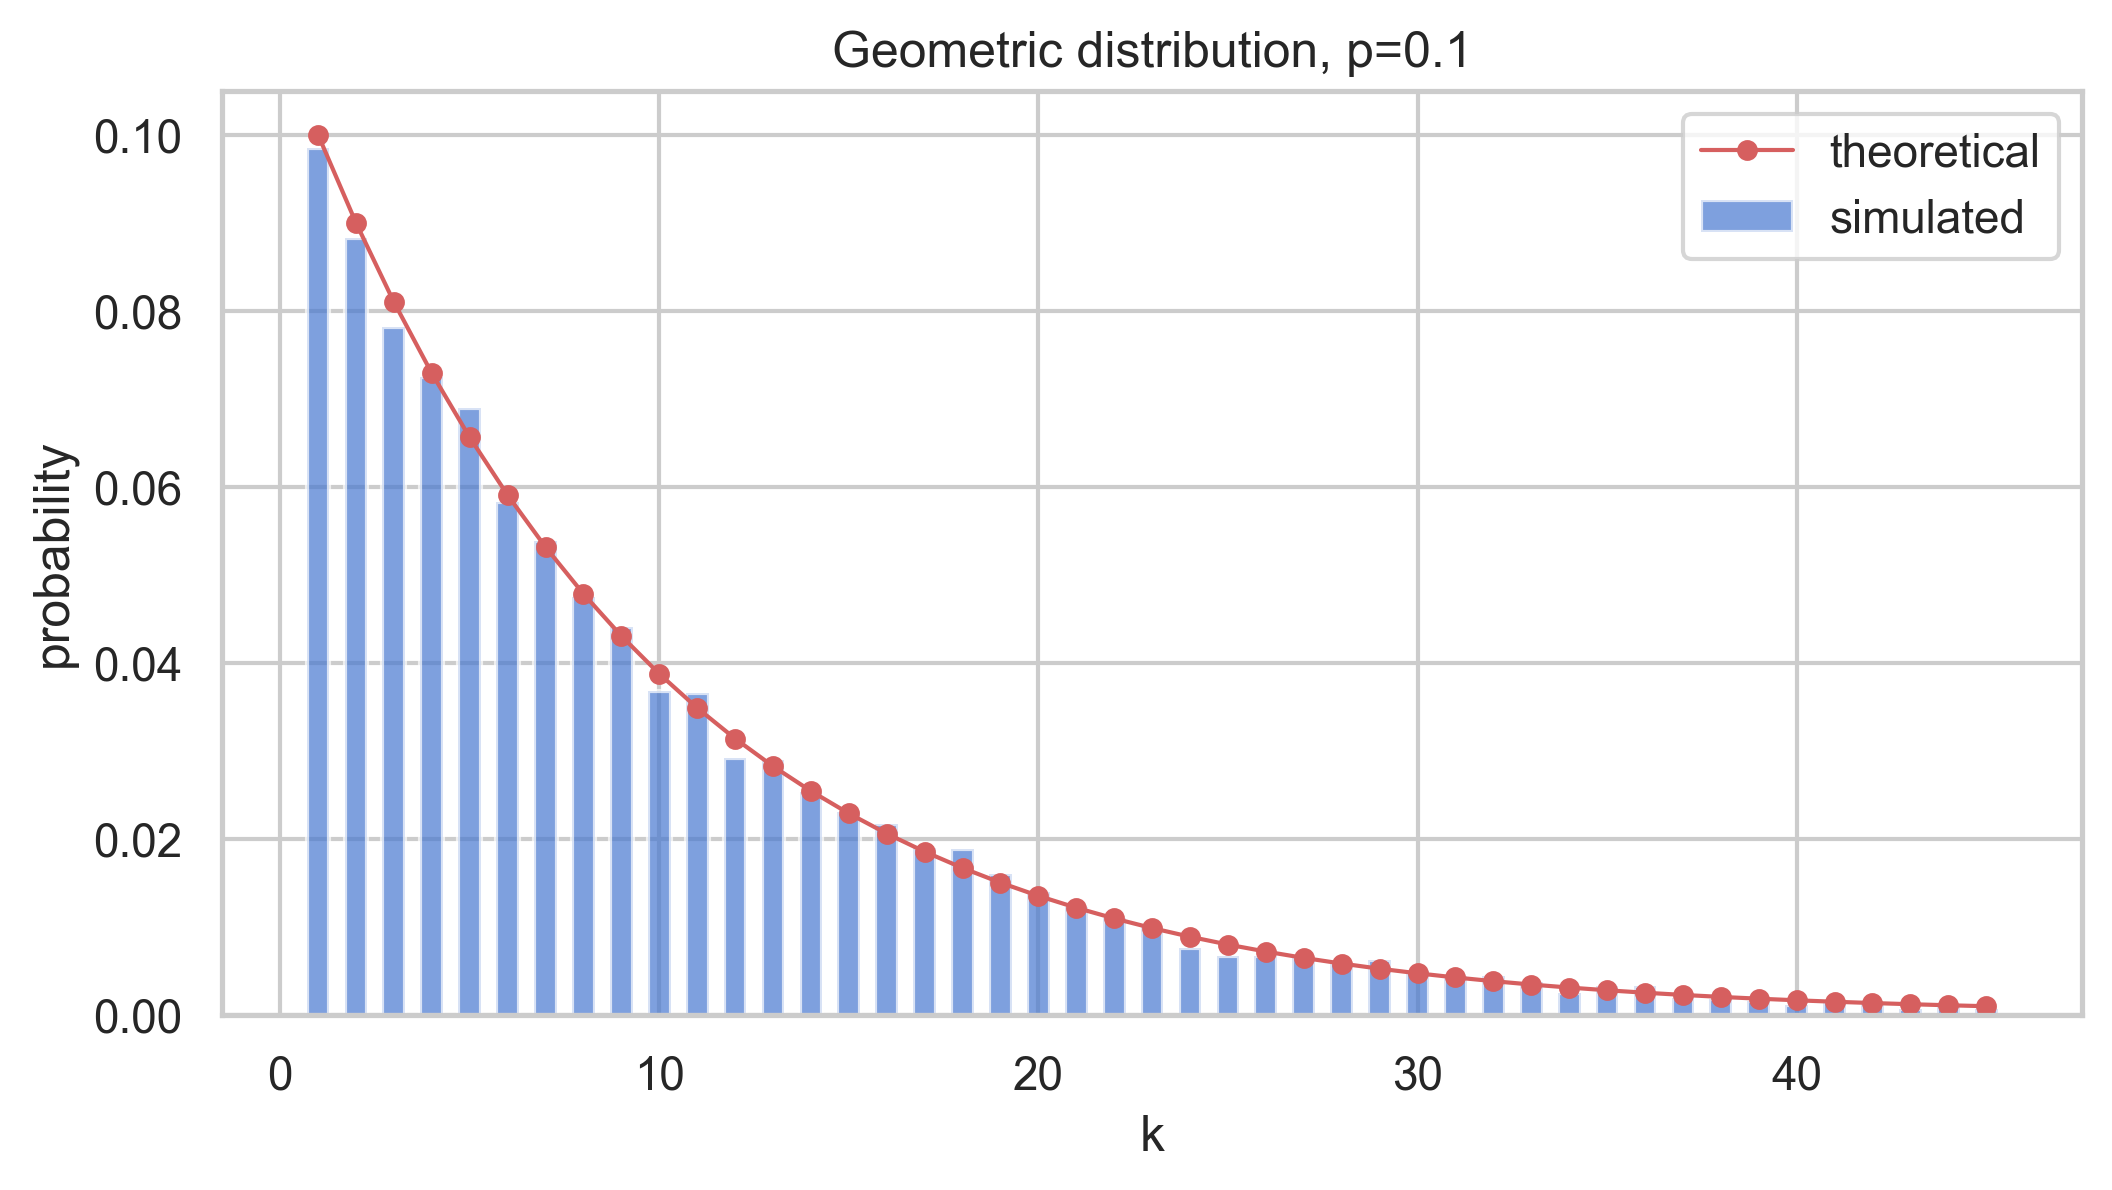
\includegraphics[width=0.32\textwidth]{plots/day2/geometric_p0.1.png}
    \hfill
    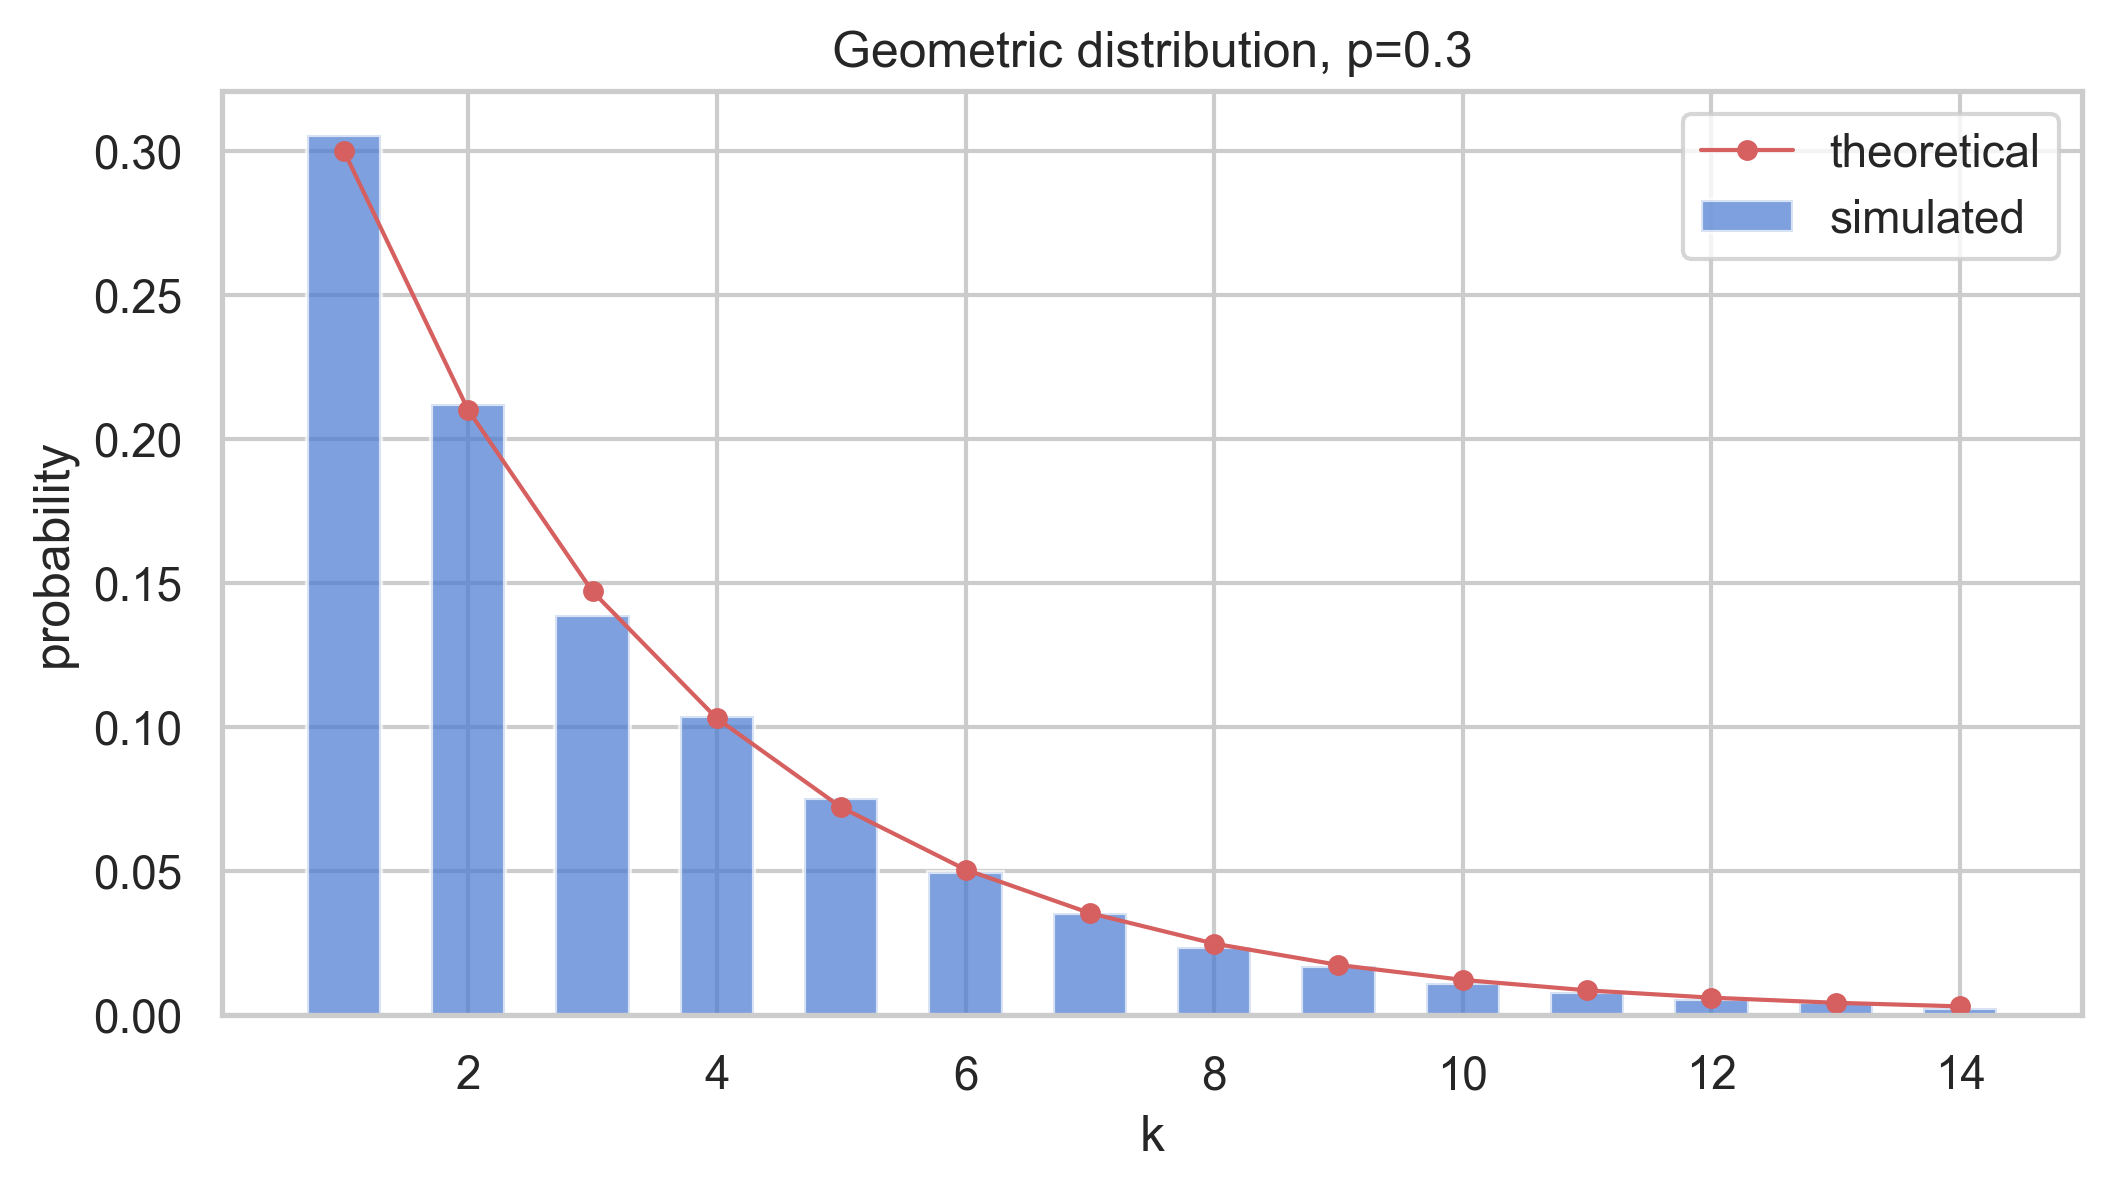
\includegraphics[width=0.32\textwidth]{plots/day2/geometric_p0.3.png}
    \hfill
    
\includegraphics[width=0.32\textwidth]{plots/day2/geometric_p0.7.png}
    \caption{Simulated (bars) vs.\ theoretical (dots) PMFs for
             $\text{Geometric}(p)$, $n = 10{,}000$.
             \textit{Left:} $p = 0.1$ --- heavy tail, spread over many values.
             \textit{Centre:} $p = 0.3$ --- moderate tail.
             \textit{Right:} $p = 0.7$ --- almost all mass at $x = 1$.}
    \label{fig:geom}
\end{figure}
 
% ================================================================
\section*{Part 2 --- Six-Point Distribution}
% ================================================================
 
The six-point distribution is a made-up discrete distribution with six
outcomes $\{1, 2, 3, 4, 5, 6\}$ and unequal probabilities --- unlike a
fair die. Outcome 6 is the most likely ($\approx 31\%$) and outcome 4 is
the least likely ($\approx 6\%$):
\begin{center}
\renewcommand{\arraystretch}{1.1}
\begin{tabular}{lrrrrrr}
    \toprule
    $x_i$               & 1              & 2              & 3             & 4              & 5             & 6              \\
    \midrule
    $\mathbb{P}(X=x_i)$ & $\tfrac{7}{48}$ & $\tfrac{5}{48}$ & $\tfrac{1}{8}$ & $\tfrac{1}{16}$ & $\tfrac{1}{4}$ & $\tfrac{5}{16}$ \\
    \bottomrule
\end{tabular}
\end{center}
 
Three sampling methods are implemented and applied to this pmf, each with
$k = 6$ outcomes:

\textbf{Crude/direct inversion} returns $X = x_i$ whenever
$F(x_{i-1}) < U \leq F(x_i)$ (slide 8), i.e.\ a binary
search of $U$ into the cumulative table (\texttt{crude\_sample}, using
\texttt{np.searchsorted}):
\begin{verbatim}
return np.searchsorted(cdf, u, side="left") + 1
\end{verbatim}

\textbf{Simple rejection} proposes $I = \lfloor kU_1 \rfloor + 1$ and accepts
it if $U_2 \leq p_I / c$ with $c = \max_i p_i$ (slide 11,
correctness proved on slide 18). Here $c = 5/16$ and $k = 6$:
\begin{verbatim}
accepted = idx[u <= probs[idx] / c]
\end{verbatim}

\textbf{Alias method} builds probability and alias tables $(F, L)$ once, then
draws $I = \lfloor kU_1 \rfloor + 1$ and returns $I$ if $U_2 \leq F(I)$, else
$L(I)$ (slides 14--16). The draw is one comparison, but the setup is the
real work, where it partitions the scaled probabilities into deficient
($<1$) and surplus ($\geq 1$) columns and pairs them off (slide 12):
\begin{verbatim}
prob = n * probs                  # column heights, mean 1
small = [i for i in range(n) if prob[i] < 1.0]
large = [i for i in range(n) if prob[i] >= 1.0]
while small and large:
    l = small.pop()
    g = large[-1]
    alias[l] = g                  # g fills the rest of l's column
    prob[g] += prob[l] - 1.0
    if prob[g] < 1.0:
        large.pop()
        small.append(g)
\end{verbatim}

The chi-square goodness-of-fit test has 6 classes, so $\mathrm{df} = 5$. We
run each method with two seeds to show that the $p$-value itself is random.

\begin{table}[h]
    \centering
    \caption{Chi-square results for the six-point distribution,
             $n = 10{,}000$. $H_0$ is rejected if $p < 0.05$.}
    \label{tab:sixpoint}
    \renewcommand{\arraystretch}{1.1}
    \begin{tabular}{lrrrr}
        \toprule
        & \multicolumn{2}{c}{Seed 42} & \multicolumn{2}{c}{Seed 69} \\
        \cmidrule(lr){2-3} \cmidrule(lr){4-5}
        Method    & $\chi^2$ & $p$-value & $\chi^2$ & $p$-value \\
        \midrule
        Crude     & $2.96$ & $0.706$ & $3.57$ & $0.613$ \\
        Rejection & $3.77$ & $0.583$ & $7.39$ & $0.193$ \\
        Alias     & $2.94$ & $0.709$ & $7.34$ & $0.196$ \\
        \bottomrule
    \end{tabular}
\end{table}

All six $p$-values exceed 0.05, but they differ noticeably between seeds for
the same sampler --- the $p$-value is itself a random draw from
$\mathcal{U}(0,1)$ under $H_0$, so some scatter is expected even when every
method is correct.

\begin{figure}[h]
    \centering
    
\includegraphics[width=0.32\textwidth]{plots/day2/sixpoint_crude.png}
    \hfill
    
\includegraphics[width=0.32\textwidth]{plots/day2/sixpoint_rejection.png}
    \hfill
    
\includegraphics[width=0.32\textwidth]{plots/day2/sixpoint_alias.png}
    \caption{Simulated (blue bars) vs.\ theoretical (orange bars) PMFs for the six-point
             distribution, seed 69, $n = 10{,}000$.
             \textit{Left:} Crude.
             \textit{Centre:} Rejection.
             \textit{Right:} Alias.}
    \label{fig:sixpoint}
\end{figure}
 
% ================================================================
\section*{Part 3 --- Method Comparison}
% ================================================================

Since all three methods are correct (verified in Part 2 via chi-squared tests), we focus on how efficiently they generate samples. With $n = 10{,}000$, the timings are dominated by noise and random variation; we therefore use $n = 1{,}000{,}000$ for a reliable comparison. Table~\ref{tab:comparison} summarises the key performance measures.

\begin{table}[h]
\centering
\caption{Performance comparison of the three generation methods at $n = 1{,}000{,}000$, seed 69.}
\label{tab:comparison}
\renewcommand{\arraystretch}{1.2}
\begin{tabular}{lrrrcc}
\toprule
Method    & $\chi^2$ & $p$-value & Time (s) & Uniforms per draw & Work per draw \\
\midrule
Crude     & 3.39     & 0.640     & 0.021    & 1                 & $O(\log k)$ \\
Rejection & 2.66     & 0.753     & 0.030    & $\approx 3.75$    & $O(1)$ per proposal \\
Alias     & 3.15     & 0.677     & 0.016    & 2                 & $O(1)$ \\
\bottomrule
\end{tabular}
\end{table}

All three methods pass the goodness-of-fit test ($p \gg 0.05$), so accuracy is not a differentiator. The alias method is fastest, requiring exactly two uniforms and $O(1)$ work per draw regardless of $k$. The crude method needs only one uniform but pays $O(\log k)$ per draw for the binary search over the CDF. The rejection method is slowest: using a discrete uniform proposal gives an acceptance probability of $1/(k \max_i p_i) = 1/(6 \cdot 5/16) \approx 0.53$, so on average $\approx 1.88$ proposals and $\approx 3.75$ uniforms are consumed per accepted sample. All three methods share $O(k)$ memory; the alias method additionally requires an $O(k)$ precomputation step to build its two lookup tables. The work-per-draw complexities are standard results looked up online rather than derived here.

\section*{Part 4 — Recommendations}

For a fixed pmf sampled many times, we recommend the alias method: it achieves $O(1)$ per draw regardless of $k$ or pmf shape, at the cost of a one-time $O(k)$ setup. When the pmf changes between draws or $k$ is small, we recommend the crude method, as it requires no setup and only one uniform per sample. We would only recommend the rejection method when the pmf is near-uniform or unnormalised (e.g.\ in MCMC), since its acceptance rate $1/(k\max_i p_i)$ degrades rapidly for peaked distributions — for this six-point pmf it already wastes nearly half its proposals. See Table~\ref{tab:recommendations} for an overview.

\begin{table}[h]
\centering
\caption{Overview of recommendations for each generation method.}
\label{tab:recommendations}
\renewcommand{\arraystretch}{1.2}
\begin{tabular}{lp{4.2cm}p{6cm}}
\toprule
Method    & Prefer when & Avoid when \\
\midrule
Crude     & Small $k$, changing pmf, or quick prototyping  & Large $k$ with many draws \\
Alias     & Fixed pmf, large $k$ or large $n$              & pmf changes frequently \\
Rejection & Near-uniform pmf or unnormalised distributions & Peaked pmf over large $k$ \\
\bottomrule
\end{tabular}
\end{table}

\newpage 
% ================================================================
\section*{Exercise 3 --- Continuous Distributions}
% ================================================================

We implement inverse-transform and Box--Muller samplers for three continuous
distributions and verify them via Kolmogorov--Smirnov (KS) tests, using the
principle that $Y = F_X^{-1}(U) \sim F_X$ for $U \sim \mathcal{U}(0,1)$
(slide 5). All
samples use $n = 10{,}000$.

% ================================================================
\section*{Part 1 --- Sampling and KS Tests}
% ================================================================

\textbf{Exponential.} Inverting $F(x) = 1 - e^{-\lambda x}$ gives
\begin{equation}
    X = -\frac{\log U}{\lambda}
    \label{eq:exp}
\end{equation}
(slide 6):
\begin{verbatim}
return -np.log(u) / lam
\end{verbatim}

\textbf{Pareto Type I.} For $F(x) = 1 - (\beta/x)^k$, $x \geq \beta$, with
$E[X] = \beta k/(k-1)$ and $V[X] = \beta^2 k / ((k-1)^2(k-2))$, inversion gives
\begin{equation}
    X = \beta U^{-1/k}
    \label{eq:pareto}
\end{equation}
(slide 7):
\begin{verbatim}
return beta / u ** (1.0 / k)
\end{verbatim}

\textbf{Normal (Box--Muller).} Two independent uniforms map to two
independent $N(0,1)$ variates via the Rayleigh-distributed radius
$R = \sqrt{-2\log U_1}$ and angle $\Theta = 2\pi U_2$:
\begin{equation}
    (Z_1, Z_2) = \big(\sqrt{-2\log U_1}\cos(2\pi U_2),\ \sqrt{-2\log U_1}\sin(2\pi U_2)\big)
    \label{eq:boxmuller}
\end{equation}
(slides 9 and 11):
\begin{verbatim}
r = np.sqrt(-2.0 * np.log(u1))
theta = 2.0 * np.pi * u2
z = np.concatenate([r * np.cos(theta), r * np.sin(theta)])
\end{verbatim}

Each sample is verified with a one-sample Kolmogorov--Smirnov (KS) test, which measures $D = \sup_x |F_n(x) - F(x)|$ --- the maximum gap between the empirical and theoretical CDFs --- without requiring any binning. The $\chi^2$ test from Exercise 2 is not used here: for continuous data, bin choices are arbitrary and degrade power, particularly in the tails. Results are in Table~\ref{tab:ks} and Figure~\ref{fig:continuous}.

\begin{table}[h]
    \centering
    \caption{KS goodness-of-fit results ($n = 10{,}000$). Sample mean is
             compared to the theoretical mean.}
    \label{tab:ks}
    \renewcommand{\arraystretch}{1.1}
    \begin{tabular}{lrrrr}
        \toprule
        Distribution & Sample mean & Theory & KS stat & $p$-value \\
        \midrule
        Exponential ($\lambda=1$) & $1.0062$ & $1.0000$ & $0.0074$ & $0.634$ \\
        Normal (Box--Muller)      & $0.0007$ & $0.0000$ & $0.0054$ & $0.928$ \\
        Pareto $k=2.05$           & $1.9723$ & $1.9524$ & $0.0082$ & $0.503$ \\
        Pareto $k=2.5$            & $1.6650$ & $1.6667$ & $0.0080$ & $0.546$ \\
        Pareto $k=3.0$            & $1.4977$ & $1.5000$ & $0.0057$ & $0.904$ \\
        Pareto $k=4.0$            & $1.3371$ & $1.3333$ & $0.0052$ & $0.949$ \\
        \bottomrule
    \end{tabular}
\end{table}

All $p$-values are well above $0.05$: every sampler reproduces its target
distribution, and the histograms in Figure~\ref{fig:continuous} track the
analytical pdfs closely, including in the heavy tail of the small-$k$ Pareto
cases.

\begin{figure}[h]
    \centering
    
\includegraphics[width=0.32\textwidth]{plots/day2/exponential.png}
    \hfill
    
\includegraphics[width=0.32\textwidth]{plots/day2/normal.png}
    \hfill
    
\includegraphics[width=0.32\textwidth]{plots/day2/pareto_all.png}
    \caption{Simulated histograms (bars) vs.\ analytical pdfs (red), $n = 10{,}000$.
             \textit{Left:} Exponential($\lambda=1$).
             \textit{Centre:} Normal via Box--Muller.
             \textit{Right:} Pareto($\beta=1$) for $k \in \{2.05, 2.5, 3, 4\}$.}
    \label{fig:continuous}
\end{figure}

% ================================================================
\section*{Part 2 --- Pareto Moments}
% ================================================================

For $\text{Pareto}(\beta, k)$, the theoretical mean and variance are
$E[X] = \beta k/(k-1)$ and $V[X] = \beta^2 k / ((k-1)^2(k-2))$ (slide 7),
defined only for
$k > 1$ and $k > 2$ respectively. Table~\ref{tab:moments} compares these to
the sample moments from the $n = 10{,}000$ draws of Part 1.

\begin{table}[h]
    \centering
    \caption{Sample vs.\ theoretical moments for Pareto($\beta=1$), $n = 10{,}000$.}
    \label{tab:moments}
    \renewcommand{\arraystretch}{1.1}
    \begin{tabular}{lrrrr}
        \toprule
        $k$ & $E[X]$ sim & $E[X]$ theory & $V[X]$ sim & $V[X]$ theory \\
        \midrule
        $2.05$ & $1.9452$ & $1.9524$ & $9.96$  & $37.19$ \\
        $2.5$  & $1.6479$ & $1.6667$ & $1.44$  & $2.22$  \\
        $3.0$  & $1.5042$ & $1.5000$ & $0.68$  & $0.75$  \\
        $4.0$  & $1.3373$ & $1.3333$ & $0.22$  & $0.22$  \\
        \bottomrule
    \end{tabular}
\end{table}

The means agree well for all $k$, but the variance at $k = 2.05$, we see a big difference: with $k - 2 = 0.05$ the denominator $(k-1)^2(k-2)$ is tiny, so
$V[X] \approx 37.19$ is very large compared to the sample value of $9.96$. The
variance of a Pareto with $k$ close to 2 is dominated by extremely rare,
extremely large draws from its heavy power-law tail; $n = 10{,}000$ samples
essentially never see them, so the sample variance severely underestimates
the true value. We verified this across 12 different seeds: sample variances
ranged from $3.8$ to $13.6$, never approaching the theoretical $37.19$, and
the spread itself reflects how much a single large draw can shift the estimate ---
seed 500 drew a maximum of $221$, giving the highest sample variance of $13.6$,
while most seeds topped out around $50$--$140$ and yielded variances of $4$--$7$.
To reliably estimate a variance this large would require $n$ in the millions.
For $k \leq 2$, $V[X]$ is theoretically infinite and no finite
sample can estimate it consistently. This motivates variance reduction
techniques covered in later exercises, which improve estimation efficiency
precisely in situations where the naive Monte Carlo estimator has high variance.

% ================================================================
\section*{Part 3 --- Normal Confidence Intervals}
% ================================================================

Using the $N(0,1)$ sampler from Part 1, we draw 100 independent samples of
$n = 10$ and construct a 95\% CI for the mean and for the variance from each.

The mean CI uses the Student-$t$ pivot rather than the normal, because $\sigma^2$
is unknown and must be estimated by $s^2$. Replacing $\sigma$ with $s$ makes the
pivot heavier-tailed than the normal --- that extra uncertainty is exactly what
the $t$-distribution accounts for:
\begin{equation}
    \bar{x} \pm t_{0.975,\,9}\sqrt{s^2/n}.
    \label{eq:ci-mean}
\end{equation}

The variance CI uses the $\chi^2$ pivot. Because the $\chi^2$ distribution is
right-skewed, the two quantile cuts are not symmetric: $\chi^2_{0.025,9} \approx 2.70$
whereas $\chi^2_{0.975,9} \approx 19.02$, so the interval is wider on the left
than on the right:
\begin{equation}
    \left(\frac{(n-1)s^2}{\chi^2_{0.975,\,9}},\ \frac{(n-1)s^2}{\chi^2_{0.025,\,9}}\right).
    \label{eq:ci-var}
\end{equation}

Coverage is the fraction of the 100 intervals that contain the true value
($\mu = 0$, $\sigma^2 = 1$).

\begin{table}[h]
    \centering
    \caption{Coverage of $100 \times 95\%$ confidence intervals from $n=10$ samples.}
    \label{tab:ci}
    \renewcommand{\arraystretch}{1.1}
    \begin{tabular}{lrr}
        \toprule
        CI for & Coverage & Expected \\
        \midrule
        Mean     & $94/100$ & $\approx 95$ \\
        Variance & $96/100$ & $\approx 95$ \\
        \bottomrule
    \end{tabular}
\end{table}

Both coverages are consistent with the nominal 95\% level: the binomial
standard error of a count out of 100 at $p=0.95$ is $\approx 2.2$, so $94$
and $96$ are both within one standard error of $95$. With only $n=10$
observations the intervals are wide --- with $t_{0.975,9} \approx 2.26$ and
$s \approx 1$, a typical half-width is $2.26/\sqrt{10} \approx 0.71$, so each
interval spans roughly $\pm 0.71$ around the sample mean. The red intervals
in Figure~\ref{fig:ci} are the ones that miss $\mu=0$.

\begin{figure}[h]
    \centering
    
\includegraphics[width=0.6\textwidth]{plots/day2/ci_mean.png}
    \caption{$100 \times 95\%$ confidence intervals for the mean, $n=10$ draws
             from the Box--Muller $N(0,1)$ sampler of Part 1. Blue intervals
             contain $\mu=0$; red intervals do not. Coverage shown in Table~\ref{tab:ci}.}
    \label{fig:ci}
\end{figure}

% ===============================================================
\section*{Part 4 --- Pareto via Composition}
% ===============================================================

Instead of generating Pareto samples directly with the inversion formula from
Part 1, the composition method breaks it into two simpler steps:
\begin{enumerate}
    \item Draw a random rate $\Lambda \sim \text{Gamma}(\text{shape}=k,\ \text{scale}=1/\beta)$.
    \item Draw $X = \beta + Y$ where $Y \sim \text{Exponential with rate } \Lambda$
          (i.e.\ mean $1/\Lambda$).
\end{enumerate}

\begin{verbatim}
lam = rng.gamma(shape=k, scale=1.0 / beta)
return beta + rng.exponential(scale=1.0 / lam)
\end{verbatim}

The result is Pareto-distributed, even though the Pareto formula was never
used directly. This works because the Pareto distribution can be written as a
mixture of exponentials with a Gamma-distributed rate: if you integrate
$\Lambda$ out of the joint density, you recover $f_X(x) = k\beta^k / x^{k+1}$,
which is exactly the Pareto pdf.

For $k = 3$, $\beta = 1$, we check that this produces the same distribution
as the inversion method from Part 1. Two KS tests confirm this: one compares
the composition samples to the theoretical Pareto pdf, the other compares
them directly to the inversion samples from Part 1. Both pass comfortably
(Table~\ref{tab:composition}).

\begin{table}[h]
    \centering
    \caption{KS tests for the composition sampler ($k = 3$, $\beta = 1$,
             $n = 10{,}000$). Both $p$-values are far above 0.05.}
    \label{tab:composition}
    \renewcommand{\arraystretch}{1.1}
    \begin{tabular}{lrr}
        \toprule
        Comparison                          & KS stat & $p$-value \\
        \midrule
        Composition vs.\ theoretical Pareto & $0.0060$ & $0.860$ \\
        Composition vs.\ inversion samples  & $0.0109$ & $0.592$ \\
        \bottomrule
    \end{tabular}
\end{table}

Both methods produce the same distribution. For Pareto, inversion is simpler
since there is a nice closed-form formula. The composition method is useful
when no such formula exists and you need to break the distribution into
simpler pieces.
\newpage
\newpage
\section*{Day 3 Exercise 4 --- Blocking System }

In this exercise we simulate a blocking system (a loss system: $m$ service units, no waiting
room) by the \emph{event-by-event principle} and estimate the fraction of
blocked customers. 


The system has $m = 10$ servers and no waiting room: a customer that arrives
when all servers are busy is lost. With mean service time $s = 8$ and mean
inter-arrival time $1/\lambda = 1$, the offered traffic is $A = \lambda s = 8$
Erlang.

The simulation maps directly onto the four core elements of a discrete event
simulation (slides 5--6): the simulation clock is the time $t$ of the current
event, the state variable is the number of busy servers \texttt{n\_busy}, the
event list is a priority queue of arrival and departure events, and the
statistical accumulator is the \texttt{blocked} counter. The main loop advances
the clock to the next event, handles it, updates the state, and schedules
future events.

Each configuration is run as $10 \times 10{,}000$ customers. The 10 runs are
treated as independent \textbf{sub-samples} (slides 16--19): each yields one
blocked-fraction estimate $\hat\theta_i$, and a 95\% confidence interval is
formed from the $t$-distribution,
\begin{equation}
    \bar\theta \pm t_{0.975,\,9}\, \frac{S_\theta}{\sqrt{10}}.
    \label{eq:ci}
\end{equation}

The exact solution is Erlang's B-formula (Lecture 5),
\begin{equation}
    B = \frac{A^m / m!}{\sum_{i=0}^{m} A^i / i!},
    \label{eq:erlangb}
\end{equation}
which is \emph{insensitive to the service-time distribution} (only the mean
matters) but \emph{requires a Poisson arrival process}. For $A = 8$, $m = 10$
it gives $B = 0.1217$, the reference value throughout.

% ================================================================
\section*{Part 1 --- Verification (Poisson Arrivals, Exponential Service)}
% ================================================================

With Poisson arrivals (exponential inter-arrival times) and
exponential service, the simulation should reproduce Erlang B. The core event
loop accepts an arrival if a server is free, otherwise counts it as blocked:
\begin{verbatim}
while events:
    t, kind, i = heapq.heappop(events)        # advance clock to next event
    if kind == ARRIVAL:
        if n_busy < m:
            n_busy += 1
            heapq.heappush(events, (t + service[i], DEPARTURE, i))
        else:
            blocked += 1                       # all servers busy -> lost
    else:
        n_busy -= 1
\end{verbatim}
Erlang B (Equation~\ref{eq:erlangb}) is evaluated with a numerically stable
recursion that avoids large factorials:
\begin{verbatim}
b = 1.0
for i in range(1, m + 1):
    b = A * b / (i + A * b)
\end{verbatim}

\begin{table}[h]
    \centering
    \caption{Part 1 result, $10 \times 10{,}000$ customers. Erlang B $= 0.1217$.}
    \label{tab:part1}
    \renewcommand{\arraystretch}{1.1}
    \begin{tabular}{lrcc}
        \toprule
        Configuration & Fraction & 95\% CI & Erlang B in CI? \\
        \midrule
        Poisson / Exponential & $0.1221$ & $[0.1184,\ 0.1258]$ & Yes \\
        \bottomrule
    \end{tabular}
\end{table}

The simulated fraction $0.1221$ matches Erlang B and its CI contains the
analytical value, verifying the event-by-event implementation.

% ================================================================
\section*{Part 2 --- Renewal Arrival Processes (Exponential Service)}
% ================================================================

Replacing the Poisson process with a renewal process (general inter-arrival
times) keeps the mean arrival rate but changes its variability.
We test Erlang($2$) inter-arrivals and a hyperexponential mixture
($p_1 = 0.8, \lambda_1 = 0.8333,\ p_2 = 0.2, \lambda_2 = 5.0$), both with mean 1.

\begin{table}[h]
    \centering
    \caption{Part 2 results (exponential service). Erlang B $= 0.1217$.}
    \label{tab:part2}
    \renewcommand{\arraystretch}{1.1}
    \begin{tabular}{lrcc}
        \toprule
        Configuration & Fraction & 95\% CI & Erlang B in CI? \\
        \midrule
        Erlang($2$) arrivals      & $0.0950$ & $[0.0911,\ 0.0990]$ & No (lower)  \\
        Hyperexponential arrivals & $0.1398$ & $[0.1347,\ 0.1449]$ & No (higher) \\
        \bottomrule
    \end{tabular}
\end{table}

Erlang B no longer applies, since it assumes Poisson arrivals. Erlang($2$)
inter-arrival times have \emph{lower} variance than exponential (more regular,
less bursty), so customers are spaced more evenly, collide less, and blocking
\emph{drops} below Erlang B. Hyperexponential inter-arrival times have
\emph{higher} variance (a mix of very short and very long gaps), so customers
cluster and blocking \emph{rises} above Erlang B. Neither CI contains $0.1217$:
blocking depends on the \emph{variability} of the arrival process, not just its
mean rate.

% ================================================================
\section*{Part 3 --- Varied Service Distributions (Poisson Arrivals)}
% ================================================================

Returning to Poisson arrivals, we vary the service-time distribution while
keeping mean $8$. For the Pareto service times the scale is set so the mean
equals $8$, i.e.\ $\beta = 8(k-1)/k$:
\begin{verbatim}
beta = 8.0 * (k - 1) / k       # so that E[X] = beta*k/(k-1) = 8
\end{verbatim}

\begin{table}[h]
    \centering
    \caption{Part 3 results (Poisson arrivals). Erlang B $= 0.1217$.}
    \label{tab:part3}
    \renewcommand{\arraystretch}{1.1}
    \begin{tabular}{lrcc}
        \toprule
        Configuration & Fraction & 95\% CI & Erlang B in CI? \\
        \midrule
        Constant service   & $0.1202$ & $[0.1157,\ 0.1247]$ & Yes        \\
        Pareto $k=1.05$     & $0.0012$ & $[0.0002,\ 0.0022]$ & No (lower) \\
        Pareto $k=2.05$     & $0.1178$ & $[0.1126,\ 0.1229]$ & Yes        \\
        Lognormal service   & $0.1208$ & $[0.1160,\ 0.1257]$ & Yes        \\
        \bottomrule
    \end{tabular}
\end{table}

Erlang B is insensitive to the service-time distribution, confirmed by
constant, Pareto $k=2.05$, and lognormal service (all matching $0.1217$).
Pareto $k=1.05$ is the exception, but it is a \emph{finite-sample bias}, not a
real violation of insensitivity. With $k = 1.05$ the mean $E[X] = \beta k/(k-1)
= 8$ is finite, but the variance is infinite ($k < 2$). Almost every draw is
tiny ($\beta \approx 0.38$), and the rare enormous values needed to lift the
sample mean to $8$ essentially never appear in $10{,}000$ draws. The
\emph{empirical} mean service time is therefore far below $8$, the system is
under-loaded, and blocking collapses to $\approx 0$.

% ================================================================
\section*{Part 4 --- Comparison}
% ================================================================

Figure~\ref{fig:comparison} shows all configurations against the Erlang B reference line. \textbf{Constant, Pareto $k = 2.05$, and lognormal service} all have their CI crossing the line, confirming that Erlang B depends only on the mean
service time, not its shape. The Part 2 CIs miss the line entirely: \textbf{Erlang(2)} arrivals are more regular than Poisson, which means customers arrive evenly spaced, so fewer hit the system at once and blocking is lower. \textbf{Hyperexponential arrivals}
are more bursty, which means customers cluster together, filling all servers, and blocking is higher. The direction of the deviation matches the variability: less variable arrivals give less blocking, more variable give more. \textbf{Pareto
$k = 1.05$} sits far below the line with the narrowest CI of all (every run is biased in the same direction). The infinite-variance distribution cannot be sampled reliably with 10{,}000
observations, so the effective mean service time is far below 8 in every run and blocking is consistently near zero.

\begin{figure}[h]
    \centering
    
\includegraphics[width=0.85\textwidth]{plots/day3/comparison.png}
    \caption{Blocked fraction with 95\% sub-sample CIs for all configurations
             against the Erlang B reference ($0.1217$, dashed). Green intervals
             contain Erlang B; red intervals deviate from it.}
    \label{fig:comparison}
\end{figure}

\newpage
\section*{Day 4}
\section*{Exercise 5}
In this exercise we explore variance reduction methods. Parts 1--4 estimate the integral $\int_0^1 e^x\,dx$ (whose exact value is $e-1 \approx 1.718282$) using four different techniques, all with comparable computer resources, aiming for 100 function evaluations for each method. Part 5 applies these ideas to the blocking system from Exercise 4, and lastly parts 7-9 deal with importance sampling.

Throughout, we report the $95\%$ confidence interval (CI) width as our measure of estimator precision. This is equivalent to reporting variance: the CI width is $2\,t_{0.975}(n-1)\,s/\sqrt{n}$, so it is a direct function of the sample variance $s^2$ and the number of observations $n$. Since both $s^2$ and $n$ differ across methods, we believe the CI width is the single most interpretable summary — it already accounts for both sources of precision.

\subsection*{Part 1 -- Crude Monte Carlo}
We use the crude Monte Carlo estimator to estimate the integral
\[
\int_0^1 e^x \, dx
\]
We draw $n$ samples $U_i \sim \operatorname{Uniform}(0,1)$ and estimate the integral as the sample mean of $e^{U_i}$,
\[
\frac{1}{n}\sum_{i=1}^n e^{U_i},
\]
with a $95\%$ confidence interval obtained from the $t$-distribution. With $n=100$ we get
\begin{center}
mean $= 1.714466$, \quad $95\%$ CI $= (1.617300,\ 1.811632)$.
\end{center}
The true value $e-1 = 1.718282$ lies inside the interval, as expected.

\subsection*{Part 2 -- Antithetic variables}
To reduce the variance we use antithetic sampling. For each $U$ we also use its antithetic counterpart $1-U$ and average the two:
\[
\frac{e^{U}+e^{1-U}}{2}.
\]
Since $U$ and $1-U$ have the same distribution, $e^{U}$ and $e^{1-U}$ also do, so $\mathbb{E}\!\left[\tfrac{1}{2}(e^{U}+e^{1-U})\right] = e-1$ and the estimator remains unbiased. Because $e^{U}$ and $e^{1-U}$ are negatively correlated, their average has reduced variance. Using $n=50$ pairs (i.e. $100$ function evaluations, comparable to Part 1) we get
\begin{center}
mean $= 1.711206$, \quad $95\%$ CI $= (1.692801,\ 1.729611)$.
\end{center}

Notice that the confidence interval is significantly tighter now, even with the sample size going from $n=100$ in part 1 to $n=50$ here. The confidence interval went from CI = (1.617300, 1.811632) which has a width of  0,1943 in part 1 to CI = (1.692801, 1.729611) which has width = 0,0368 in part 2 indicating that variance reduction was successfully achieved by incorporating the antithetic variable.

\subsection*{Part 3 -- Control variate}
Next we use a control variate. This is a technique where we add a related random variable, with its mean subtracted so that the added term $Z-\mathbb{E}[Z]$ satisfies $\mathbb{E}\!\left[Z-\mathbb{E}[Z]\right]=0$ and the estimator thus remains unbiased. The idea is then to scale this term by a constant $c$ chosen to maximize the variance reduction (i.e.\ minimize the overall variance). The final added term is thus $c\,(Z-\mathbb{E}[Z])$. The optimal value for the constant is given as
\[
c = -\frac{\operatorname{Cov}(X_i, Z_i)}{\operatorname{Var}(Z_i)},
\]
where $X$ is the target and $Z$ is the control variate. We choose $Z = U$, since it is strongly correlated with $e^{U}$ and is very simple to evaluate. In the simulation $c$ is estimated empirically from the sample by
\begin{lstlisting}[language=Python, basicstyle=\ttfamily\small]
c = -np.cov(X, Z, ddof=1)[0, 1] / np.var(Z, ddof=1)
\end{lstlisting}
which gives $c \approx -1.688$.

We use $n=100$, since there is only one function evaluation per iteration, keeping
the computational resources comparable to the previous parts. Using this control
variate approach we obtain
\begin{center}
mean $= 1.716209$, \quad $95\%$ CI $= (1.704551,\ 1.727866)$.
\end{center}
The width of the CI is thus further reduced compared to Part 2 (antithetic variables), and the interval still contains the true value, as expected. It is worth noting that both methods have essentially the same theoretical per-observation variance ($\approx 0.0039$), so the improvement here is partly due to $n$: control variates yield $100$ independent observations from $100$ evaluations, whereas antithetic variables yield only $50$ pairs. The methods are not quite on equal footing in that sense, even though the total number of function evaluations is the same.

\subsection*{Part 4 -- Stratified sampling}
Stratified sampling is a simple idea: instead of drawing $U$ uniformly on $[0,1)$, we split $[0,1)$ into $k$ subintervals of equal length and draw one sample from each, repeating $n/k$ times so that we still obtain $n$ total samples. 
Within stratum $j$ the draw is confined to that subinterval,
\[
U_j = \frac{j+V}{k}, \qquad V \sim \operatorname{Uniform}(0,1).
\]

This reduces variance because the samples can no longer cluster by chance in one region of the domain. There is now no variance between different strata but only some possible variance within the strata itself.
Now each iteration of the loop results in one estimator value:
\[
Y_i = \frac{1}{k}\sum_{j=1}^{k} e^{U_j},
\]
We repeat this $n/k$ times and thus get $n/k$ estimators. Therefore the mean and confidence interval are calculated based on this composite estimator. 
With $n=100$ and $k=10$ we get
\begin{center}
mean $= 1.722733$, \quad $95\%$ CI $= (1.715688,\ 1.729779)$.
\end{center}

Once again, we managed to reduce the width of the confidence interval even below the confidence interval from part 2 and 3, indicating that stratified sampling works well for variance reduction, at least for this problem.

\subsection*{Comparison of Parts 1--4.}
Table~\ref{tab:vr14} compares the confidence interval widths of the four estimators at comparable computer resources. All three variance reduction methods clearly outperform crude Monte Carlo, and out of our methods and approaches, stratified sampling gives the narrowest interval, followed by the control variate and then antithetic sampling.

\begin{table}[h]
\centering
\caption{$95\%$ CI widths for estimates of $\int_0^1 e^x\,dx$ at comparable compute.}
\label{tab:vr14}
\begin{tabular}{lrr}
\toprule
Method & CI width & Reduction vs.\ crude \\
\midrule
Crude (Part 1)        & $0.1943$ & --- \\
Antithetic (Part 2)   & $0.0368$ & $\sim 5\times$ \\
Control variate (Part 3) & $0.0233$ & $\sim 8\times$ \\
Stratified (Part 4)   & $0.0141$ & $\sim 14\times$ \\
\bottomrule
\end{tabular}
\end{table}

\begin{figure}
    \centering
    
\includegraphics[width=0.7\linewidth]{plots//day4/ci_comparison.png}
    \caption{95\% confidence intervals for $\int_0^1 e^x\,dx$ across the four methods at comparable compute (100 function evaluation each). The red dashed line marks the true value $e-1$.}
    \label{fig:ci_comparison}
\end{figure}

\subsection*{Part 5 -- Control variates on the blocking system}
We now apply variance reduction to the blocking system from Exercise 4, using a control variate to reduce the variance of the estimated blocking fraction.

We use the sum of the inter-arrival times $S$ as the control variate. Its expectation is known: with $n$ customers and mean inter-arrival time $1$ we have $\mathbb{E}[S] = n$. Intuitively, when arrivals are spread out (large $S$) the system is less loaded and fewer customers are blocked, so $S$ is negatively correlated with the blocking fraction $B$ and is a natural control variate.

We first perform $100$ runs to estimate the optimal coefficient
\[
c = \frac{\operatorname{Cov}(B, S)}{\operatorname{Var}(S)},
\]
and then run a fresh batch of simulations to find the estimate $Y_i = B_i - c\,(S_i - n)$:

\begin{lstlisting}[language=Python, basicstyle=\ttfamily\small]
Bs, Ss, Ys = [], [], []
n = 10000
n_reps = 100
for i in range(n_reps):
    arrival_fn = lambda: np.random.exponential(1.0)
    service_fn = lambda: np.random.exponential(8.0)
    B_i, S_i = simulate_cv(arrival_fn, service_fn, m=10, n=n)
    Bs.append(B_i)
    Ss.append(S_i)
    Ys.append(B_i - c * (S_i - n))

mean = np.mean(Ys)
std = np.std(Ys, ddof=1)
half_width = scipy.stats.t.ppf(0.975, df=n_reps-1) * std / np.sqrt(n_reps)
\end{lstlisting}

The results of the simulation run are shown in Table~\ref{tab:part5_results}, with the Erlang B reference value $0.121661$ for comparison. The control variate reduces the CI width by about $20\%$. The reduction is less than what we saw in parts 1-4, but it is still a reasonable reduction in variance for no extra per-simulation cost (beyond a short pilot run to estimate the $c$ constant).

\begin{table}[h]
\centering
\caption{Means and CI widths for the simulated blocking system.}
\label{tab:part5_results}
\begin{tabular}{lrrr}
\toprule
Method & Mean & CI width & Reduction vs.\ crude \\
\midrule
Crude (no CV)   & $0.121796$ & $0.002216$ & --- \\
Control variate & $0.121185$ & $0.001767$ & $\sim 1.25\times$ \\
\bottomrule
\end{tabular}
\end{table}

\subsection*{Part 7 -- Importance sampling for $P(Z > a)$} We estimate $P(Z > a)$ for $Z \sim N(0,1)$. First we use crude Monte Carlo, and then importance sampling with a proposal density that is normal with mean $a$ and variance $\sigma^2$, for different values of $a$, $\sigma^2$, and sample size $n$. The results are shown in Table~\ref{tab:is7}.

\begin{table}[h]
\centering
\caption{Crude vs.\ importance sampling for $P(Z>a)$. True values:
$P(Z>2) = 2.28\times10^{-2}$, $P(Z>4) = 3.17\times10^{-5}$.}
\label{tab:is7}
\begin{tabular}{cclrr}
\toprule
$n$ & $a$ & Method & Mean & CI width \\
\midrule
\multirow{8}{*}{$100$}
 & \multirow{4}{*}{$2$} & Crude            & $3.00\times10^{-2}$ & $6.80\times10^{-2}$ \\
 &                      & IS, $\sigma^2=1$ & $2.15\times10^{-2}$ & $1.37\times10^{-2}$ \\
 &                      & IS, $\sigma^2=2$ & $2.10\times10^{-2}$ & $1.47\times10^{-2}$ \\
 &                      & IS, $\sigma^2=3$ & $1.56\times10^{-2}$ & $1.36\times10^{-2}$ \\
\cmidrule(l){2-5}
 & \multirow{4}{*}{$4$} & Crude            & $0.00$              & $0.00$ \\
 &                      & IS, $\sigma^2=1$ & $3.67\times10^{-5}$ & $3.16\times10^{-5}$ \\
 &                      & IS, $\sigma^2=2$ & $2.40\times10^{-5}$ & $2.64\times10^{-5}$ \\
 &                      & IS, $\sigma^2=3$ & $3.09\times10^{-5}$ & $3.12\times10^{-5}$ \\
\midrule
\multirow{8}{*}{$1000$}
 & \multirow{4}{*}{$2$} & Crude            & $2.10\times10^{-2}$ & $1.78\times10^{-2}$ \\
 &                      & IS, $\sigma^2=1$ & $2.41\times10^{-2}$ & $4.36\times10^{-3}$ \\
 &                      & IS, $\sigma^2=2$ & $2.10\times10^{-2}$ & $5.03\times10^{-3}$ \\
 &                      & IS, $\sigma^2=3$ & $2.32\times10^{-2}$ & $6.24\times10^{-3}$ \\
\cmidrule(l){2-5}
 & \multirow{4}{*}{$4$} & Crude            & $0.00$              & $0.00$ \\
 &                      & IS, $\sigma^2=1$ & $3.03\times10^{-5}$ & $7.92\times10^{-6}$ \\
 &                      & IS, $\sigma^2=2$ & $2.96\times10^{-5}$ & $1.02\times10^{-5}$ \\
 &                      & IS, $\sigma^2=3$ & $3.16\times10^{-5}$ & $1.11\times10^{-5}$ \\
\midrule
\multirow{8}{*}{$10000$}
 & \multirow{4}{*}{$2$} & Crude            & $2.22\times10^{-2}$ & $5.78\times10^{-3}$ \\
 &                      & IS, $\sigma^2=1$ & $2.22\times10^{-2}$ & $1.35\times10^{-3}$ \\
 &                      & IS, $\sigma^2=2$ & $2.33\times10^{-2}$ & $1.72\times10^{-3}$ \\
 &                      & IS, $\sigma^2=3$ & $2.26\times10^{-2}$ & $1.91\times10^{-3}$ \\
\cmidrule(l){2-5}
 & \multirow{4}{*}{$4$} & Crude            & $0.00$              & $0.00$ \\
 &                      & IS, $\sigma^2=1$ & $3.10\times10^{-5}$ & $2.60\times10^{-6}$ \\
 &                      & IS, $\sigma^2=2$ & $3.17\times10^{-5}$ & $3.21\times10^{-6}$ \\
 &                      & IS, $\sigma^2=3$ & $3.19\times10^{-5}$ & $3.63\times10^{-6}$ \\
\bottomrule
\end{tabular}
\end{table}

It is remarkable how much better importance sampling performs. Already at $n=100$ it captures the rare events and produces a much narrower confidence interval than crude Monte Carlo (e.g. $1.47\times10^{-2}$ vs.\ $6.80\times10^{-2}$ for $a=2$). So for essentially the same compute, importance sampling gives far lower variance.

The effect is even more dramatic for the rare event $a=4$: crude Monte Carlo returns exactly $0$ for $n \le 1000$ because it never draws a sample beyond $4$, whereas importance sampling estimates the true probability $3.17\times10^{-5}$ relatively accurately already at $n=100$ and very accurately at the larger sample sizes. Finally, if performance is measured by confidence interval width, the smallest variance $\sigma^2 = 1$ performed best overall among the proposals tried, having the lowest CI width in 5 out of 6 comparisons.

\subsection*{Part 8 -- Importance sampling with an exponential proposal}
We estimate the integral
\[
\theta = \int_0^1 e^x \, dx
\]
using importance sampling. Following the notation from the lecture,
we write the quantity of interest as
\[
\theta = \mathbb{E}[h(X)] = \int_{-\infty}^{\infty} h(x)\,f(x)\,dx,
\qquad
h(x) = e^x,
\qquad
f(x) = \mathbf{1}_{\{0 \le x \le 1\}},
\]
where $h$ is the integrand and $f$ is the $\operatorname{Uniform}(0,1)$ density. The indicator makes
$f$ zero outside $[0,1]$, so this reproduces the original integral.

Instead of sampling from $f$, we sample from the proposal density
\[
g(x) = \lambda e^{-\lambda x}\]
Since $g(x) > 0$ wherever $f(x) > 0$, the identity from slide~27 gives
\[
\theta = \int h(x)\frac{f(x)}{g(x)}\,g(x)\,dx
       = \mathbb{E}\!\left[h(X)\frac{f(X)}{g(X)}\right],
\]
with estimator $\hat{\theta}_{IS} = \tfrac{1}{n}\sum_{i=1}^n h(X_i)\frac{f(X_i)}{g(X_i)}$.
The importance sampling random variable is therefore
\[
W = h(X)\frac{f(X)}{g(X)}
  = \frac{e^X\,\mathbf{1}_{\{0\le X\le 1\}}}{\lambda e^{-\lambda X}}
  = \frac{1}{\lambda}e^{(1+\lambda)X}\mathbf{1}_{\{0\le X\le 1\}}.
\]
Since $X \sim \operatorname{Exp}(\lambda)$ is always non-negative,
$\mathbf{1}_{\{0\le X\le 1\}} = \mathbf{1}_{\{X\le 1\}}$.

To find the optimal $\lambda$ we analyze $\operatorname{Var}(W)$. Since the estimator is unbiased, $\mathbb{E}[W]=\int_0^1 e^x\,dx = e-1$, so
\[
\operatorname{Var}(W)
=
\mathbb{E}[W^2]-\mathbb{E}[W]^2
=
\mathbb{E}[W^2]-(e-1)^2 .
\]
Now we calculate $\mathbb{E}[W^2]$
\[
\mathbb{E}[W^2]
=\int_{-\infty}^\infty W(x)^2 g(x)\,dx
=\int_0^1 \frac{e^{2x(1+\lambda)}}{\lambda^2}\,\lambda e^{-\lambda x}\,dx
=\frac{1}{\lambda}\int_0^1 e^{(2+\lambda)x}\,dx ,
\]
hence
\[
\mathbb{E}[W^2]
=\frac{1}{\lambda}\left[\frac{e^{(2+\lambda)x}}{2+\lambda}\right]_0^1
=\frac{e^{2+\lambda}-1}{\lambda(2+\lambda)},
\qquad
\operatorname{Var}(W)
=\frac{e^{2+\lambda}-1}{\lambda(2+\lambda)}-(e-1)^2 .
\]
The variance of the estimator is $\operatorname{Var}(\hat{I}_{IS}) =
\tfrac{1}{n}\operatorname{Var}(W)$. Since $1/n$ and $(e-1)^2$ is independent of $\lambda$,
minimising the variance is equivalent to minimising
$\frac{e^{2+\lambda}-1}{\lambda(2+\lambda)}$. Done numerically, this gives
\footnote{ChatGPT-5.5 was used to assist with the derivation.}

\[
\boxed{\lambda^* \approx 1.3548}
\]

with minimum variance $\operatorname{Var}(W) \approx 3.1288$.

Running the simulation gives the results in Table~\ref{tab:is8}.

\begin{table}[h]
\centering
\caption{Crude MC vs.\ exponential importance sampling for $\int_0^1 e^x\,dx$
($n=10{,}000$). True value $e-1 = 1.718282$.}
\label{tab:is8}
\begin{tabular}{lrr}
\toprule
Estimator & Mean & CI width \\
\midrule
Crude MC                       & $1.717034$ & $0.019294$ \\
IS, $\lambda=0.500$            & $1.645545$ & $0.093913$ \\
IS, $\lambda=1.000$            & $1.693668$ & $0.072518$ \\
IS, $\lambda^*=1.355$          & $1.732042$ & $0.070012$ \\
IS, $\lambda=2.000$            & $1.710978$ & $0.075783$ \\
IS, $\lambda=5.000$            & $1.629328$ & $0.196602$ \\
\bottomrule
\end{tabular}
\end{table}

The simulation confirms the analysis: among the exponential proposals, the narrowest interval is indeed obtained at $\lambda^* \approx 1.355$, with CI width $0.070$. However, this is still about $3.6\times$ \emph{wider} than crude Monte Carlo ($0.019$). This matches the analytical result, $\operatorname{Var}(W) \approx 3.13$ at $\lambda^*$ versus a crude MC variance of only $\approx 0.242$. So importance sampling with an exponential distribution does \emph{not} reduce the variance here. The reason is that the exponential density is decreasing on $[0,1]$, whereas the integrand $e^x$ is increasing, so the proposal is the wrong shape and over-weights the region where the integrand is smallest.

\subsection*{Part 9 -- Pareto first-moment distribution}
\newpage
\section*{Day 5}
\section*{Exercise 6}

In this exercise we apply Markov chain Monte Carlo (MCMC) to three problems:
a truncated Poisson distribution (Part 1), a truncated bivariate distribution
where direct sampling is awkward but the conditional distributions are
tractable (Part 2), and a Bayesian inference problem with a log-normal prior
(Part 3). For all discrete cases we verify the samplers using a $\chi^2$
goodness-of-fit test against the exact target distribution.

\subsection{Part 1: Truncated Poisson via Metropolis Hastings}

The target is the distribution:
\begin{equation}
    P(i) = c\frac{A^{i}}{i!}, \qquad i=0,1,\dots,m,
\end{equation}
with values similar to part 4 ( $A=8$, $m=10$). The normalizing constant $c$ depends on $m$ and is not
needed by Metropolis Hastings since the acceptance ratio only involves
$g(i)=A^{i}/i!$:
\begin{equation}
    \alpha(i,j) \;=\; \min\!\left(1,\;\frac{g(j)}{g(i)}\right)
                = \min \left(1, \frac{A^j/j!}{A^i/i!}\right).
\end{equation}
We use a symmetric proposal distribution, h(i,j) namely, random-walk proposal on the integers, $j = i \pm 1$ with
equal probability, and reject any move outside $\{0,\dots,m\}$. The core loop
is:
\begin{lstlisting}[language=Python]
samples = [initial_state]
for _ in range(n):
    current_state  = samples[-1]
    proposed_state = current_state + np.random.choice([-1, 1])
    if proposed_state < lo or proposed_state > hi:
        samples.append(current_state); continue
    acceptance_prob = min(1, g(proposed_state) / g(current_state))
    if np.random.random() < acceptance_prob:
        samples.append(proposed_state)
    else:
        samples.append(current_state)
\end{lstlisting}
Figure~\ref{fig:mh_part1} shows the empirical distribution after $10^{5}$ MH
steps thinned by a factor of $10$, (Done to reduce correlation between 1-lag samples, tool used in model-based machine learning course 42186). A $\chi^2$ goodness-of-fit test against the
exact pmf, pooling bins with expected count below $5$, gives
$\chi^2 = 2.919$ on $9$ degrees of freedom with $p = 0.967$, so we
comfortably fail to reject the null hypothesis that the samples come from
the truncated Poisson.

\begin{figure}[H]
    \centering
    
\includegraphics[width=0.6\linewidth]{plots/day5/metropolis_hastings_samples.png}
    \caption{Metropolis--Hastings samples from the truncated Poisson with
    $A=8$, $m=10$.}
    \label{fig:mh_part1}
\end{figure}

\subsection{Part 2: Joint truncated distribution}

We now target the joint
\begin{equation}
    P(i,j) \;=\; c\,\frac{A_{1}^{i}}{i!}\,\frac{A_{2}^{j}}{j!},
    \qquad 0 \le i+j \le m,
\end{equation}
with $A_{1}=A_{2}=4$ and $m=10$. We sample this in two ways: coordinate-wise
Metropolis--Hastings and Gibbs sampling. (A direct joint random-walk proposal
that perturbs both coordinates simultaneously by $\pm 1$ was implemented but
discarded -- it mixes poorly because every step couples the two coordinates,
and it cannot easily reach states near the boundary $i+j=m$.)

\paragraph{Coordinate-wise Metropolis--Hastings.}
At each iteration we pick one coordinate uniformly at random and propose a
$\pm 1$ step on it; the other coordinate is held fixed. Proposals that violate
$i,j\ge 0$ or $i+j>m$ are rejected. The acceptance ratio is the same
factorial expression as in Part~1.
\begin{lstlisting}[language=Python]
p = np.random.random()
if p < 0.5:
    proposed_i, proposed_j = curr_i + np.random.choice([-1, 1]), curr_j
else:
    proposed_i, proposed_j = curr_i, curr_j + np.random.choice([-1, 1])
\end{lstlisting}

\paragraph{Gibbs sampling.}
The full conditional of $i$ given $j$ is itself a truncated Poisson on
$\{0,\dots,m-j\}$ proportional to $A_{1}^{i}/i!$, and symmetrically for $j$
given $i$. We sample this conditional directly by enumerating its pmf on the
allowed support:
\begin{equation}
    P(A_1 = i | A_2 = j) = \frac{P(A_1=i, A_2=j)}{\sum_i'^{m-j}P(A_1=i, A_2=j)} = \frac{\frac{4^i 4^j}{i! j!}}{\sum_{i'}^{m-j}\frac{4^{i'} 4^j}{{i'}! j!}} = \frac{\frac{4^i}{i!}}{\sum_{i'}^{m-j}\frac{4^{i'}}{{i'}!}} 
\end{equation}
Because every proposal is drawn from the exact conditional, there is no
accept/reject step; every sweep updates both coordinates.

Figure~\ref{fig:mh_part2} and Figure~\ref{fig:gibbs_part2} show the
distribution of the sum $i+j$ for the two samplers. The $\chi^2$ test against
the exact joint pmf gives $\chi^2 = 55.54$, $p = 0.79$ on $65$ d.o.f. for
the coordinate-wise MH sampler and $\chi^2 = 61.01$, $p = 0.62$ on $65$
d.o.f. for the Gibbs sampler. Both samplers fail to reject the null at any
reasonable significance level, with the MH sampler giving a marginally higher
$p$-value here.

\begin{figure}[H]
    \centering
    
\includegraphics[width=0.6\linewidth]{plots/day5/metropolis_hastings_samples_part2.png}
    \caption{Coordinate-wise Metropolis--Hastings samples: distribution of
    $i+j$ with $A_{1}=A_{2}=4$, $m=10$.}
    \label{fig:mh_part2}
\end{figure}

\begin{figure}[H]
    \centering
    
\includegraphics[width=0.6\linewidth]{plots/day5/gibbs_samples_part2.png}
    \caption{Gibbs sampling: distribution of $i+j$ with $A_{1}=A_{2}=4$,
    $m=10$.}
    \label{fig:gibbs_part2}
\end{figure}

\subsection{Part 3: Bayesian inference with a log-normal prior}

We consider the model $X_{i}\mid (\Theta,\Psi)\sim N(\Theta,\Psi)$ where the
prior on $(\Xi,\Gamma)=(\log\Theta,\log\Psi)$ is bivariate normal with
standard-normal marginals and correlation $\rho=\tfrac{1}{2}$, so that
$(\Theta,\Psi)$ has the log-normal density given in the problem statement.

\subsubsection*{Sampling the prior}

For a bi-variate standard normal with correlation $\rho$, the relation between the 2 variates is defined as: 
\begin{equation}
    Y = \rho X + \sqrt{1-\rho^2} = \frac{X}{2} + \frac{\sqrt{2}}{2} Z
\end{equation}
where $X, Z \sim \mathcal{N}(0,1)$. So the generative story becomes: 
\begin{itemize} 
    \item for sample in samples draw $\Gamma_i, Z_i \sim \mathcal{N}(0,1), \mathcal{N}(0,1)$
    \item for each sample i draw $\Xi_i = \frac{\Gamma_i}{2} + \frac{\sqrt{3}}{2} Z_i$
    \item  $\Theta = e^\Xi, \Psi = e^\Gamma$
\end{itemize}

The Gaussian $(\Xi,\Gamma)$ and the
exponentiated $(\Theta,\Psi)$ are shown in
Figures~\ref{fig:prior_log} and \ref{fig:prior}.

\begin{figure}[H]
    \centering
    
\includegraphics[width=0.55\linewidth]{plots/day5/log_prior_samples.png}
    \caption{Prior samples in log-space: $(\Xi,\Gamma)$ from a standard
    bivariate normal with $\rho=0.5$.}
    \label{fig:prior_log}
\end{figure}

\begin{figure}[H]
    \centering
    
\includegraphics[width=0.55\linewidth]{plots/day5/prior_samples.png}
    \caption{Prior samples $(\Theta,\Psi)=(e^{\Xi},e^{\Gamma})$ on the
    original scale.}
    \label{fig:prior}
\end{figure}

\subsubsection*{(b) Simulating observations}

We now draw $(\theta, \psi)$ once from the prior then, we simulate the likelihood 
$X_{1},\dots,X_{n}\sim N(\theta,\psi)$. Figure~\ref{fig:data} shows the
$n=10$ observations used in part~(d).

\begin{figure}[H]
    \centering
    
\includegraphics[width=0.55\linewidth]{plots/day5/gaussian_samples_theta_psi.png}
    \caption{Simulated observations $X_{1},\dots,X_{10}\sim N(\theta,\psi)$
    for the prior draw $(\theta,\psi)$.}
    \label{fig:data}
\end{figure}

\subsubsection*{(c) Posterior derivation}

We shall now consider how the posterior distribution looks like for this setup: 
We first remember ourselves that the posterior is proportional to the joint density with some constant. In other words the posterior distribution is proportional to the likelihood times the prior. 
\begin{equation}
    P(\Theta, \Psi | X) = \frac{P(\Theta, \Psi, X)}{\iint P(\Theta, \Psi, X) d\theta d\psi} =
    \frac{P(X|\Theta, \Psi) P(\Theta, \Psi)}{\iint P(\Theta, \Psi, X) d \theta d \psi} \propto P(X|\Theta, \Psi) P(\Theta, \Psi) 
\end{equation}
\begin{equation}
     P(X|\Theta, \Psi) P(\Theta, \Psi) = \left( \prod_{i=1}^n  P(X_i|\Theta, \Psi) \right) P(\Theta, \Psi) = \left( \prod_{i=1}^n \mathcal{N}(\Theta, \Psi) \right) f(\Theta, \Psi)
\end{equation}
\begin{equation}
    \left(\prod_{i=1}^n \frac{1}{\sqrt{2 \pi \psi}}  e^{- \frac{(x_i -\theta)^2}{2 \psi}} \right) \frac{1}{2 \pi \theta \psi \sqrt{1-\rho^2}} e^{ -\frac{\log (\theta)^2-2 \rho \log (\theta) \log (\psi\psi)+\log (\psi)^2}{2\left(1-\rho^2\right)}}
\end{equation}
\begin{equation}
    (2 \pi \psi)^{- \frac{n}{2}}  e^{-\frac{1}{2 \psi} \sum_{i=1}^n (x_i -\theta)^2} \frac{1}{2 \pi \theta \psi \sqrt{1-\rho^2}} e^{ -\frac{\log (\theta)^2-2 \rho \log (\theta) \log (\psi\psi)+\log (\psi)^2}{2\left(1-\rho^2\right)}}
\end{equation}
Since we consider the density proportional to the posterior we can remove the constants: 
\begin{equation}
    P(\Theta, \Psi | X) \propto \psi^{- \frac{n}{2}} \frac{1}{\theta \psi} e^{-\frac{1}{2 \psi} \sum_{i=1}^n (x_i -\theta)^2} e^{ -\frac{\log (\theta)^2-2 \rho \log (\theta) \log (\psi\psi)+\log (\psi)^2}{2\left(1-\rho^2\right)}}
\end{equation}

We have now derived a density proportional to the posterior distribution. That we are able to evaluate from. With a proposal distribution of 
\begin{equation}
    h(\theta, \psi) = \mathcal{N}(0, \Sigma)
\end{equation}
We can now make use of the MH algorithm to sample from the posterior distribution. 

\subsubsection*{(d) Metropolis--Hastings on the posterior}

We use a coordinate-wise random-walk proposal with Gaussian increments of
standard deviation $\Sigma=1$, at each step one of $\theta,\psi$ is
"randomly walked" by $\mathcal{N}(0,\Sigma^{2})$, the other is held fixed. Any proposal with $\theta\le 0$ or $\psi\le 0$ is rejected immediately (these states have zero prior mass under the log-normal prior). The acceptance ratio is the posterior ratio
\begin{equation}
    \alpha = \min\left(1,\frac{P(\theta', \psi' | \{x_i\}_{i=1}^{10}) }
    {P(\theta, \psi | \{x_i\}_{i=1}^{10})} \right)
\end{equation}

Figure~\ref{fig:posterior} shows the posterior samples for $n=10$
observations: the chain concentrates sharply around the true $(\theta,\psi)$
used to generate the data, as expected once the likelihood begins to dominate
the prior.

\begin{figure}[H]
    \centering
    
\includegraphics[width=0.55\linewidth]{plots/day5/posterior_samples_xobs10.png}
    \caption{Posterior samples from Metropolis--Hastings with $n=10$
    observations. NOTE: n in title is n_samples for $\theta, \psi$}
    \label{fig:posteriorx10}
\end{figure}



\subsubsection*{(e) Larger samples and numerical stability}
\begin{figure}[H]
    \centering
    
\includegraphics[width=0.55\linewidth]{plots/day5/posterior_samples.png}
    \caption{Posterior samples from Metropolis--Hastings with $n=100$
    observations. NOTE: n in title is n_samples for $\theta, \psi$}
    \label{fig:posterior}
\end{figure}

Repeating with $n=\{100, 1000\}$ for n = 100 it was fine, but when n = 1000 we reach a numerical issue in the likelihood
$(2\pi\psi)^{-n/2}\exp\!\bigl(-\tfrac{1}{2\psi}\sum(X_{i}-\theta)^{2}\bigr)$
is zero almost everywhere in the state space, and the acceptance
ratio $0/0$ leaves the chain stuck or wandering between disconnected modes. as is seen in \autoref{fig:posterior n 1000 numerical issue}: 

\begin{figure}[H]
    \centering
    
\includegraphics[width=0.55\linewidth]{plots/day5/posterior_samples_xobs1000.png}
    \caption{Posterior samples from Metropolis--Hastings with $n=1000$
    observations. NOTE: n in title is n_samples for $\theta, \psi$}
    \label{fig:posterior n 1000 numerical issue}
\end{figure}


one way to solve this is the sampling in log-space:
\begin{equation}
    \alpha = min(1, \exp(\log(P(\theta', \psi' | X) - \log(P(\theta, \psi | X)))
\end{equation}
and accept iff $ U < \alpha$ for $U\sim\mathrm{Unif}(0,1)$. With this
change the sampler is well-behaved at $n=1000$ and concentrates even more tightly around the true parameter values (Figure~\ref{fig:posterior_log}). 

\begin{figure}[H]
    \centering
    
\includegraphics[width=0.55\linewidth]{plots/day5/log_posterior_samples.png}
    \caption{Posterior samples using the log-posterior implementation with
    $n=1000$ observations.}
    \label{fig:posterior_log}
\end{figure}

A thing to notice regarding the proposal distribution. In this case we chose a symmetric distribution namely the gaussian centered at 0, however choosing the correct variance $\Sigma$ is important as well. We conducted a test to see the effect of 3 different values $\Sigma = [0.01, 1, 50]$

Recall the chosen proposal distribution was.
\begin{equation}
    h(x,x') = x + \varepsilon, \quad  \varepsilon \sim \mathcal{N}(0,\Sigma),
\end{equation}
It was applied coordinate-wise to one of $(\theta,\psi)$ per step. The step size
$\Sigma$ determines how efficiently the chain explores the state space. 

\subsubsection*{Too small a step ($\Sigma=0.01$)}

With a very small proposal variance almost every move is accepted, but each
move barely changes the state. The chain moves in tiny increments and
takes too long to traverse the posterior. The result is
visible in Figure~\ref{fig:sigma_small}: the empirical density is patchy and multimodal-looking, as is seen by the contours.

\begin{figure}[H]
    \centering
    \begin{subfigure}[t]{0.48\linewidth}
        
\includegraphics[width=\linewidth]{plots/day5/posterior_samples_xobs10sigma_001.png}
        \caption{$n=10$ observations.}
    \end{subfigure}
    \hfill
    \begin{subfigure}[t]{0.48\linewidth}
        
\includegraphics[width=\linewidth]{plots/day5/log_posterior_samples_sigma_001.png}
        \caption{$n=1000$ observations (log-posterior).}
    \end{subfigure}
    \caption{Posterior samples with $\Sigma=0.01$. The chain takes tiny
    steps; high acceptance but very slow mixing. The empirical density is
    rough and shows spurious local structure.}
    \label{fig:sigma_small}
\end{figure}

\subsubsection*{Well-tuned step ($\Sigma=1$)}

A proposal standard deviation seems to be of the order as the posteriors' deviations and thereby the empirical density is smooth and unimodal in both axes
(Figure~\ref{fig:sigma_one}). The $n=1000$ panel is tightly concentrated around the true $(\theta,\psi)$.

\begin{figure}[H]
    \centering
    \begin{subfigure}[t]{0.48\linewidth}
        
\includegraphics[width=\linewidth]{plots/day5/posterior_samples_xobs10.png}
        \caption{$n=10$ observations.}
    \end{subfigure}
    \hfill
    \begin{subfigure}[t]{0.48\linewidth}
        
\includegraphics[width=\linewidth]{plots/day5/log_posterior_samples.png}
        \caption{$n=1000$ observations (log-posterior).}
    \end{subfigure}
    \caption{Posterior samples with $\Sigma=1$. Smooth, unimodal empirical
    densities; the chain mixes well across the support.}
    \label{fig:sigma_one}
\end{figure}

\subsubsection*{Too large a step ($\Sigma=50$)}

When $\Sigma$ is much larger than the posterior standard deviation, almost every proposal lands far in the tail of the target where the density is low compared to the current state, and the acceptance ratio is therefore small. The chain stays put for long stretches, occasionally jumping to a random distant point that happens to be accepted. The samples in Figure~\ref{fig:sigma_large} are sparse and noisy, the histograms are spiky and the contours just look like noise

\begin{figure}[H]
    \centering
    \begin{subfigure}[t]{0.48\linewidth}
        
\includegraphics[width=\linewidth]{plots/day5/posterior_samples_xobs10_sigma50.png}
        \caption{$n=10$ observations.}
    \end{subfigure}
    \hfill
    \begin{subfigure}[t]{0.48\linewidth}
        
\includegraphics[width=\linewidth]{plots/day5/log_posterior_samples_sigma50.png}
        \caption{$n=1000$ observations (log-posterior).}
    \end{subfigure}
    \caption{Posterior samples with $\Sigma=50$. Almost every proposal is
    rejected; the chain spends long stretches at the same state and the
    resulting density is sparse and noisy.}
    \label{fig:sigma_large}
\end{figure}

Through these examples we have demonstrated how we can sample a complex posterior distribution with the metropolis hastings algorithm and that tuning the variance of the proposal distribution matters. As the number of observations increase the likelihood plays a more important role and the posterior looks gaussian for both parameters. For a large number of observation we had to ensure numerical stablity by doing MH on the log-posterior distribution.
\newpage
\newpage
\section*{Day 6 Exercises}
\section*{Exercise 7 --- Simulated Annealing for the TSP}

The Travelling Salesman Problem (TSP) asks for the shortest cyclic tour
visiting $N$ cities exactly once and returning to the starting city. The
tour cost is
\begin{equation}
    f(S) = \sum_{i=1}^{N} D\bigl[S_i,\, S_{i+1 \bmod N}\bigr],
    \label{eq:tourcost}
\end{equation}
where $S$ is a permutation of cities and $D[i,j]$ is the travel cost from
city $i$ to city $j$. Since the number of candidate tours grows as $O(N!)$,
exact optimisation is infeasible for large $N$, and we instead approximate
the optimum using \emph{simulated annealing} (SA).

% ================================================================
\section*{Part 1a --- Circle Sanity Check}
% ================================================================

We place $N = 20$ points evenly on a unit circle, using the Euclidean
distance as $D[i,j]$. The optimal tour is the regular polygon with
analytically known perimeter $2N\sin(\pi/N)$, which provides a ground-truth
check of the implementation.

SA is a stochastic optimisation algorithm that uses the Metropolis--Hastings
acceptance rule with a decreasing temperature schedule. At each iteration
$k$, a neighbouring tour $Y$ is proposed from the current tour $X$. If the
cost decreases ($\Delta = f(Y) - f(X) \le 0$) the move is accepted;
otherwise it is accepted with probability $\exp(-\Delta / T_k)$. This
controlled acceptance of uphill moves prevents the algorithm from getting
trapped in local optima (slide 11), with exploration narrowing as
$T_k \to 0$ (slide 12):
\begin{verbatim}
delta = route_cost(y, D) - route_cost(x, D)
if delta <= 0 or rng.random() < np.exp(-delta / cooling(k)):
    x, cost_x = y, cost_y
    if cost_x < best_cost:
        best_route, best_cost = x.copy(), cost_x
\end{verbatim}
Proposals are generated by swapping two randomly selected cities on the
route, as suggested in the exercise:
\begin{verbatim}
def swap_proposal(route, rng):
    new_route = route.copy()
    i, j = rng.choice(len(route), size=2, replace=False)
    new_route[i], new_route[j] = new_route[j], new_route[i]
    return new_route
\end{verbatim}
We use the cooling schedule $T_k = 1/\sqrt{1+k}$ and run for
$N_{\mathrm{iter}} = 20{,}000$ iterations, tracking the best tour seen.

\begin{table}[h]
    \centering
    \caption{Circle sanity check, $N = 20$.}
    \label{tab:circle}
    \renewcommand{\arraystretch}{1.1}
    \begin{tabular}{lr}
        \toprule
        & Cost \\
        \midrule
        Initial (random) route            & $28.2882$ \\
        Best route (SA)                   & $6.2574$  \\
        Polygon perimeter $2N\sin(\pi/N)$ & $6.2574$  \\
        \bottomrule
    \end{tabular}
\end{table}

SA recovers the exact optimum to four decimal places, confirming the
implementation is correct. Figure~\ref{fig:circle} illustrates the
improvement: the initial route crosses itself many times, while the final
route is the non-self-intersecting regular polygon.

\begin{figure}[H]
    \centering
    
\includegraphics[width=0.8\textwidth]{plots/day6/circle_sanity.png}
    \caption{Initial (left) and final (right) routes for 20 points on a unit
             circle. The final route is the non-crossing regular polygon.}
    \label{fig:circle}
\end{figure}

% ================================================================
\section*{Part 1b --- Random Points}
% ================================================================

Now that we have passed the sanity check, we try a more interesting case and draw $N = 20$ points uniformly in the unit square, again using Euclidean distance as $D[i,j]$, the swap proposal, and $T_k = 1/\sqrt{1+k}$ cooling.
As shown in Table~\ref{tab:random}, the tour cost is reduced by 55\% from
the random initial route. Figure~\ref{fig:random} shows that most of the
improvement occurs within the first ${\sim}2{,}000$ iterations, after which
the trajectory flattens as the temperature cools and fewer uphill moves are
accepted.

\begin{table}[H]
    \centering
    \caption{Random points, $N = 20$.}
    \label{tab:random}
    \renewcommand{\arraystretch}{1.1}
    \begin{tabular}{lr}
        \toprule
        & Cost \\
        \midrule
        Initial (random) route & $9.5276$ \\
        Best route (SA)        & $4.3009$ \\
        \bottomrule
    \end{tabular}
\end{table}

\begin{figure}[H]
    \centering
    
\includegraphics[width=0.8\textwidth]{plots/day6/random_route.png}
    \caption{Final route (left) and cost-vs-iteration trajectory (right) for
             20 uniform random points in the unit square.}
    \label{fig:random}
\end{figure}
\newpage
% ================================================================
\section*{Part 2 --- General Cost Matrix}
% ================================================================

We now modify the program to work with general travel costs. We load the
$20 \times 20$ asymmetric cost matrix from Learn and initialise SA from the
identity route $0, 1, \ldots, 19$ with the swap proposal and
$T_k = 1/\sqrt{1+k}$ cooling. Since Equation~\eqref{eq:tourcost} already
uses directional lookups $D[S_i, S_{i+1}]$, no modification is needed to
handle asymmetry. The cost computation is vectorised as:
\begin{verbatim}
def route_cost(route, D):
    return D[route, np.roll(route, -1)].sum()
\end{verbatim}
SA reduces the tour cost from $3{,}404$ to $1{,}339$, with best route
(1-indexed towns):
\[
    13,\ 18,\ 7,\ 17,\ 3,\ 20,\ 11,\ 16,\ 10,\ 9,\
    19,\ 15,\ 4,\ 1,\ 8,\ 5,\ 2,\ 14,\ 12,\ 6.
\]

To experiment with different design choices, we implement a
second cooling schedule $T_k = 1/\ln(2+k)$ and a segment-reversal (2-opt)
move, which reverses a randomly chosen contiguous sub-sequence of the tour:
\begin{verbatim}
def reverse_proposal(route, rng):
    i, j = sorted(rng.choice(len(route), size=2, replace=False))
    new_route = route.copy()
    new_route[i:j+1] = new_route[i:j+1][::-1]
    return new_route
\end{verbatim}
We cross both proposals with both cooling schedules and average the best
cost over 5 independent seeds, as reported in Table~\ref{tab:experiment}.

\begin{table}[h]
    \centering
    \caption{Mean best cost over 5 seeds, $N_{\text{iter}} = 20{,}000$.}
    \label{tab:experiment}
    \renewcommand{\arraystretch}{1.1}
    \begin{tabular}{llr}
        \toprule
        Cooling & Proposal & Mean best cost \\
        \midrule
        $1/\sqrt{1+k}$ & Swap    & $1201.0$ \\
        $1/\sqrt{1+k}$ & Reverse & $811.8$  \\
        $1/\ln(2+k)$   & Swap    & $1201.0$ \\
        $1/\ln(2+k)$   & Reverse & $811.8$  \\
        \bottomrule
    \end{tabular}
\end{table}

The proposal mechanism is the dominant factor: segment-reversal achieves a
32\% lower cost than random swaps regardless of the cooling schedule, while
the two cooling schedules perform identically within the iteration budget
used. This is consistent with the practical considerations on candidate
generation (slide 14): the quality of the neighborhood structure drives
performance more than the precise cooling rate. 

\newpage
\section*{Exercise 8 --- Bootstrapping}


In this exercise we apply the \emph{bootstrap}, a non-parametric technique for
estimating the variance of a statistical estimator when no analytical
expression is available (slides 6--7). The idea is to replace the unknown
distribution $F$ by the empirical distribution $F_e$ built from the observed
data, simulate many resampled datasets, and read off the variability of the
resulting estimates.

% ================================================================
\section*{Part 1 --- Ross Exercise 13}
% ================================================================

For i.i.d.\ $X_1,\dots,X_n$ with unknown mean $\mu$ and constants $a<b$ we
want to estimate
\begin{equation}
    p = P\Bigl\{a < \tfrac{1}{n}\textstyle\sum_{i=1}^{n} X_i - \mu < b\Bigr\}.
    \label{eq:p13}
\end{equation}

\textbf{(a)} The empirical distribution $F_e$ assigns mass $1/n$ to each
observation (slide 8),
\begin{equation}
    F_e(x) = \frac{1}{n}\sum_{i=1}^{n} \mathbf{1}\{x_i \le x\}.
    \label{eq:edf}
\end{equation}
Since $nF_e(x)\sim\mathrm{Binomial}(n,F(x))$ we have
$\mathbb{E}[F_e(x)] = F(x)$ and
$\mathbb{V}[F_e(x)] = F(x)(1-F(x))/n$, so $F_e$ is an unbiased and
consistent surrogate for $F$ (slide 10). Drawing from $F_e$ amounts to sampling
with replacement from the data (Ross, p.\ 147).

Under $F_e$ the population mean is the sample mean $\bar x$, so $\bar x$ plays
the role of the unknown $\mu$. The bootstrap estimate of $p$ is then: draw $k$
bootstrap samples of size $n$ with replacement, compute each bootstrap mean
$\bar X^*_i$, and estimate $p$ by the proportion falling within $(a,b)$ of
$\bar x$:
\begin{equation}
    \hat p = \frac{1}{k}\sum_{i=1}^{k}
             \mathbf{1}\bigl\{a < \bar X^*_i - \bar x < b\bigr\}.
    \label{eq:phat}
\end{equation}
The resampling is implemented as:
\begin{verbatim}
def bootstrap_replicates(data, statistic, k, rng):
    n = len(data)
    samples = rng.choice(data, size=(k, n), replace=True)
    return np.apply_along_axis(statistic, 1, samples)
\end{verbatim}

\textbf{(b)} We estimate p, with bootstrap samples $n=10$, data $56,101,78,67,93,87,64,72,80,69$, $a=-5$,
$b=5$ and $k=10{,}000$:

\begin{table}[H]
    \centering
    \caption{Bootstrap estimate of $p$ in Equation~\eqref{eq:p13}.}
    \label{tab:part1}
    \renewcommand{\arraystretch}{1.1}
    \begin{tabular}{lr}
        \toprule
        Quantity & Value \\
        \midrule
        $\bar x$  & $76.70$ \\
        $\hat p$  & $0.7658$ \\
        \bottomrule
    \end{tabular}
\end{table}

So the bootstrap probability that the sample mean of $10$ observations lands
within $\pm 5$ of the true mean is approximately $0.77$.
Figure~\ref{fig:part1} shows the bootstrap distribution of
$\bar X^* - \bar x$ with the interval $[a,b]$ shaded.

\begin{figure}[H]
    \centering
    
\includegraphics[width=0.6\textwidth]{plots/day6/ex13_bootstrap_mean.png}
    \caption{Bootstrap distribution of $\bar X^* - \bar x$ ($k=10{,}000$). The
             shaded band is $[a,b]=[-5,5]$; its mass is $\hat p = 0.7658$.}
    \label{fig:part1}
\end{figure}

% ================================================================
\section*{Part 2 --- Ross Exercise 15}
% ================================================================

We want to estimate $\mathrm{Var}(S^2)$, the variance of the sample variance
$S^2 = \sum_{i=1}^{n}(X_i - \bar X)^2/(n-1)$, for $n=15$ and data
$5,4,9,6,21,17,11,20,7,10,21,15,13,16,8$. No convenient closed form exists, so
we apply the bootstrap (slide 11): resample with replacement, recompute
$S^{2*}$ for each bootstrap sample, and take the sample variance of the
$k=10{,}000$ replicates:
\begin{equation}
    \bar\theta^* = \frac{1}{k}\sum_{i=1}^{k}\hat\theta^*_i,
    \qquad
    \hat{\mathbb{V}}[\hat\theta] =
        \frac{1}{k-1}\sum_{i=1}^{k}
        \bigl(\hat\theta^*_i - \bar\theta^*\bigr)^2.
    \label{eq:boot-var}
\end{equation}
This is implemented as seen below and our results are reported in table~\ref{tab:part2}:
\begin{verbatim}
def bootstrap_variance(data, statistic, k, rng):
    replicates = bootstrap_replicates(data, statistic, k, rng)
    return statistic(data), replicates.var(ddof=1)
\end{verbatim}

\begin{table}[H]
    \centering
    \caption{Bootstrap estimate of $\mathrm{Var}(S^2)$.}
    \label{tab:part2}
    \renewcommand{\arraystretch}{1.1}
    \begin{tabular}{lr}
        \toprule
        Quantity & Value \\
        \midrule
        Observed $S^2$ & $34.31$ \\
        $\widehat{\mathrm{Var}}(S^2)$ & $57.92$ \\
        \bottomrule
    \end{tabular}
\end{table}


% ================================================================
\section*{Part 3 --- Sample mean vs.\ sample median}
% ================================================================

We write a program that takes a sample as input and returns the sample median
together with a bootstrap estimate of its variance based on $k=100$ replicates
(Equation~\eqref{eq:boot-var}). We then run it on $n=200$ observations from a
Pareto($\beta=1, k=1.05$) distribution, sampled by inversion
$X = \beta\, U^{-1/k}$ (as on Day 2).

\textbf{1--3)} We compute the sample mean and median, and bootstrap the
variance of each. Our results are reported in table ~\ref{tab:part3}:

\begin{table}[H]
    \centering
    \caption{Bootstrap variance of the mean and the median,
             Pareto($\beta=1, k=1.05$), $n=200$, $k=100$.}
    \label{tab:part3}
    \renewcommand{\arraystretch}{1.1}
    \begin{tabular}{lrrr}
        \toprule
        Estimator & Estimate & Bootstrap variance & Bootstrap std.\ error \\
        \midrule
        Sample mean   & $7.39$ & $8.642$ & $2.940$ \\
        Sample median & $2.06$ & $0.018$ & $0.136$ \\
        \bottomrule
    \end{tabular}
\end{table}

\textbf{4)} The sample median is far more precise  than the sample
mean for this distribution, with a bootstrap variance roughly $8.642 / 0.018 \approx 480$ times
smaller.

\textbf{5)} The difference can be explained by the underlying distribution. For
$k=1.05$ the Pareto mean is finite ($\beta k/(k-1)=21$) but the variance is
\emph{infinite} ($k<2$), so the distribution is extremely heavy-tailed. A few
rare, very large observations dominate the sample mean, making it both imprecise
and biased low for this sample size ($7.39$ versus the true mean of $21$). The
median depends only on the central order statistics and is unaffected by extreme
tail values, giving a much smaller and more stable bootstrap variance. This is a good example of when the bootstrap is useful (slide 5), since
there is no simple formula for the variance of the median.

\end{document}